\documentclass[conference]{IEEEtran}
\usepackage{pifont}
\usepackage{graphicx}
\usepackage{amsmath}
\usepackage{mybeamer}
%\usepackage{draftwatermark}
\usepackage{hyperref}
\hypersetup{
    colorlinks=true,
    linkcolor=blue,
    filecolor=magenta,      
    urlcolor=cyan,
}



\newcommand{\eg}{\mbox{{\em e.g.}}}
\newcommand{\ie}{\mbox{{\em i.e.}}}
\newcommand{\viz}{\mbox{{\em viz.}}}

\title{\Large {\bf Protocol-Guided Analysis of Post-silicon
  Traces Under Limited Observability}}

 \author{\large Hao Zheng$^1$, Yuting Cao$^1$, Sandip Ray$^2$, Jin Yang$^2$ \\
 $^1$Dept. of Computer Science and Eng., University of South Florida, Tampa, Fl 33620. USA. \\
 $^2$Strategic CAD Labs, Intel Corporation, Hillsboro, OR 97124.  USA.}

\begin{document}

\maketitle

\begin{abstract}
We consider the problem of reconstructing system-level
behavior of an SoC design from a partially observed signal
trace.  Solving this problem is a critical activity in
post-silicon validation, and currently depends primarily on
human creativity and insights.  In this paper, we provide an
algorithm to automatically infer system-level transactions
from incomplete, ambiguous, and noisy trace data.  We
demonstrate the approach on a multicore virtual platoform
developed within the GEM5 environment.
\end{abstract}

\section{Introduction}

Post-silicon validation makes use of pre-production silicon
integrated circuit (IC) to ensure that the fabricated system
works as desired under actual operating conditions with real
software.  Since the silicon executes at target clock speed,
post-silicon executions are billions of times faster than
RTL simulations, and even provide speed-up of several orders
of magnitude over other pre-silicon platforms (\eg, FPGA,
system-level emulation, etc.).  This makes it possible to
explore deep design states which cannot be exercised in
pre-silicon, and identify errors missed during pre-silicon
validation and debug.  Post-silicon validation is a critical
component of the design validation life-cycle for modern
microprocessors and SoC designs.  Unfortunately, it is also
a highly complex component, performed under aggressive
schedules and accounting for more than $50\%$ of the overall
design validation cost~\cite{Patra2007}.  Consequently, it is crucial to
develop techniques for streamlining and automating
post-silicon validation activities.

A key component of post-silicon validation of SoC designs is
to correlate traces from silicon execution with the intended
system-level transactions.  An SoC design is typically
composed of a large number of pre-designed hardware or
software blocks (often referred to as ``intellectual
properties'' or ``IPs'') that coordinate through complex
protocols to implement the system-level behavior.  Any
execution trace of the system involves a large number of
interleaved instances of these protocols.  For example,
consider a smartphone executing a usage scenario where the
end-user browses the Web while listening to music and
sending and receiving occasional text messages.  Typical
post-silicon validation use-cases involve exercising such
scenarios.  An execution trace would involve activities from
the CPU, audio controller, display controller, wireless
radio antenna, etc., reflecting the interleaved execution of
several communication protocols.  On the other hand, due to
observability limitations, only a small number of
participating signals can be actually traced during silicon
execution.  Furthermore, due to electrical perturbations,
silicon data can be noisy, lossy, and ambiguous.
Consequently, it is non-trivial to identify all
participating protocols and pinpoint the interleaving that
results in an observed trace.

In this paper, we consider the problem of reconstructing
protocol-level behavior from silicon traces in SoC designs.
Given a collection of system-level communication protocols
and a trace of (partially observed) hardware signals, our
approach infers, with a certain measure of confidence, the
protocol instances (and their interleavings) being exercised
by the trace.  The approach is based on a formalization of
system-level transactions via labeled Petri-Nets, which are
capable of describing sequencing, concurrency, and choices
over system events.  We develop algorithms to infer
system-level transactions from traces with missing, noisy,
and ambiguous signal values.  We demonstrate our approach on
a multicore virtual platform constructed within the GEM5
environment~\cite{Binkert2011}.


\begin{figure*}[tb]
\begin{center}
\begin{tabular}{cc}
\begin{minipage}{3in}
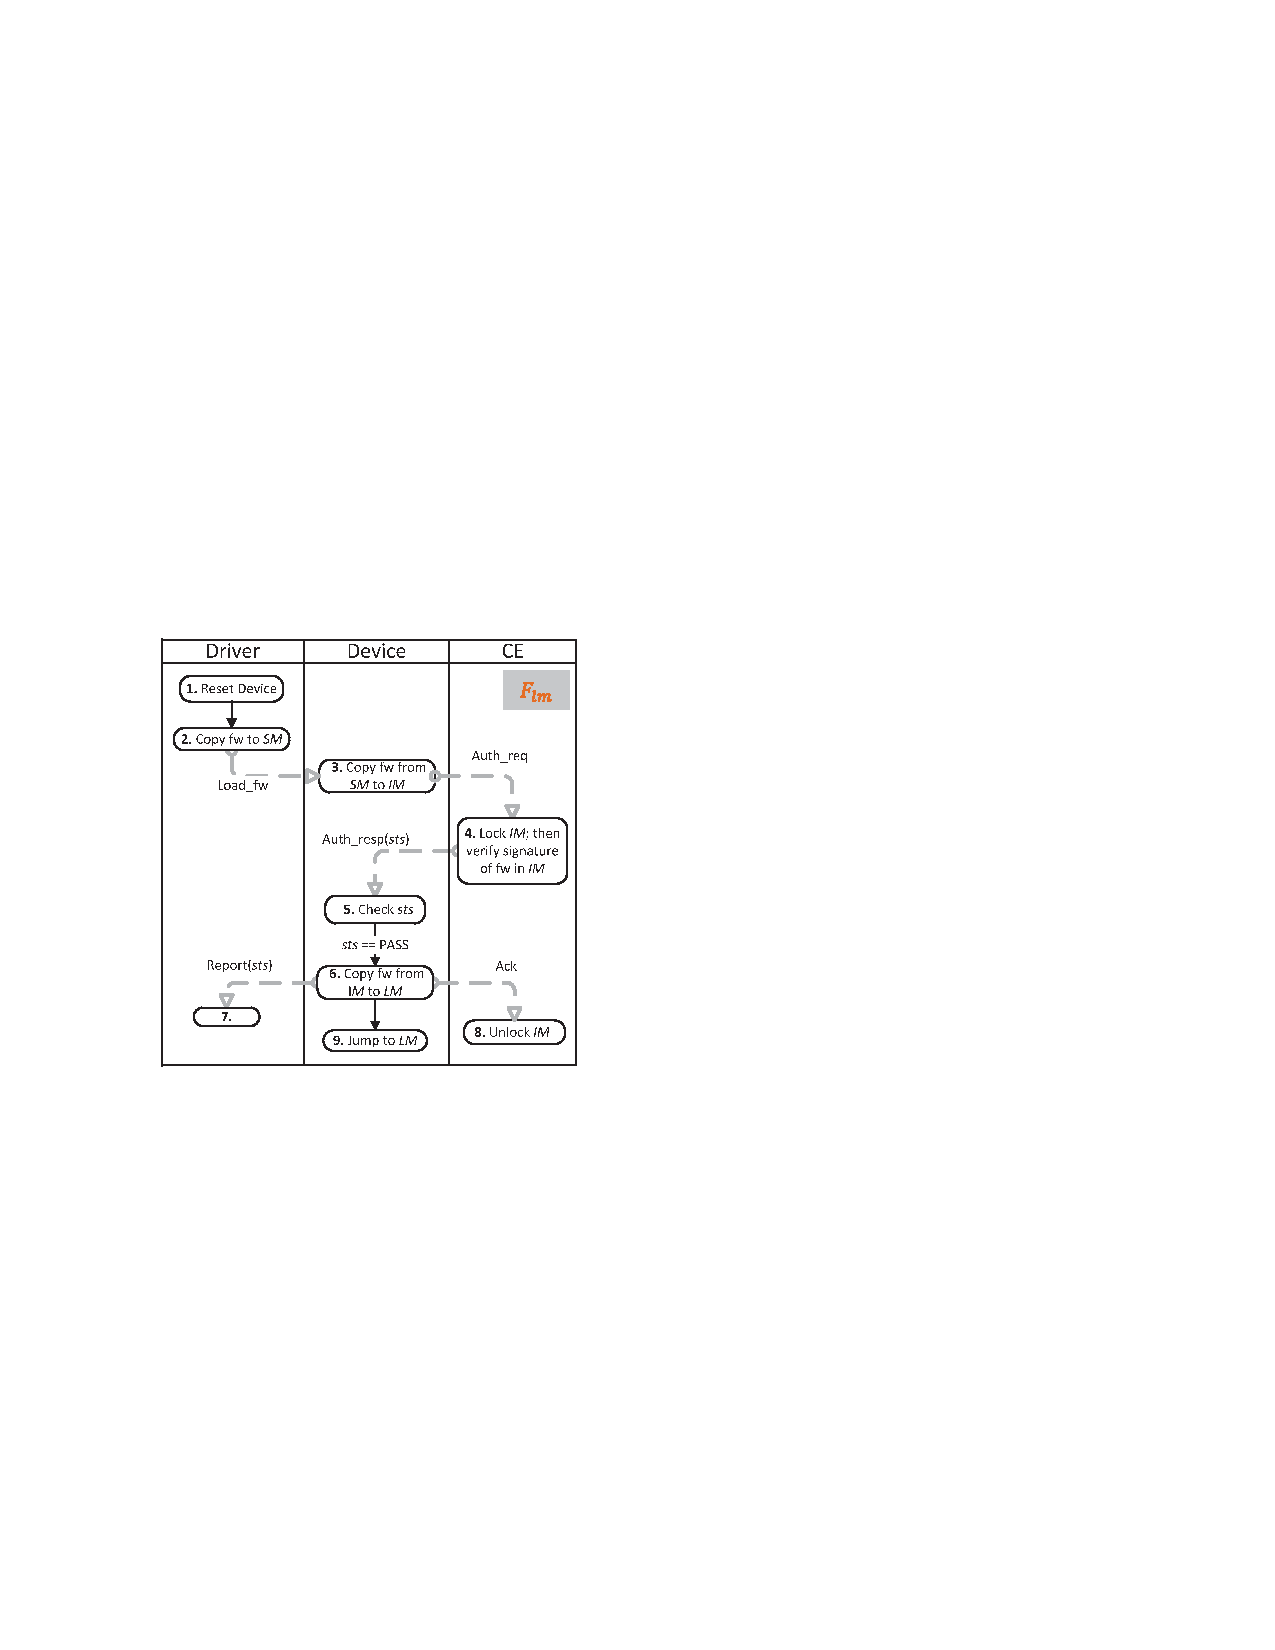
\includegraphics[height=2in]{figures/bpmn-flow-ex}
\end{minipage}
&
\begin{minipage}{3in}
\resizebox{2.4in}{!}{
\begin{tikzpicture}[node distance=3cm, auto,>=latex', thick]
\tikzset{rectbox/.style={rectangle, draw, align=flush center,thick, minimum size = 6mm}}
\tikzset{circ/.style={circle, draw,thick}}
\tikzset{terminal/.style={circle, draw,line width=.8mm}}
\tikzset{weight3/.style={line width=.3mm}}
	% Nodes:
	\node[circ]		(p1) 		at (0,0) {$p_1$};
	\node[rectbox]	(t1)	at	($(p1) + (0,-1.1)$) {$t_1:\langle {\tt Driver:Device:Load} \_fw\rangle$};
	\node[circ] 	(p2) 		at ($(t1) + (0,-1.1)$) {$p_2$};
	\node[rectbox]	(t2)	at	($(p2) + (0,-1.1)$) {$t_2:\langle {\tt Device:CE:Auth\_req} \rangle$};
	\node[circ] 	(p3) 		at ($(t2) + (0,-1.1)$) {$p_3$};
	\node[rectbox]	(t3)	at	($(p3) + (0,-1.1)$) {$t_3:\langle {\tt CE:Device:Auth\_resp}\rangle$};
	\node[circ] 	(p4) 		at ($(t3) + (0,-1.1)$) {$p_4$};
	\node[rectbox]	(t4)	at	($(p4) + (-3,-1.1)$) {$t_4:\langle {\tt Device:Driver:Report} \rangle$};
	\node[rectbox]	(t5)	at	($(p4) + (3,-1.1)$) {$t_5:\langle {\tt Device:CE:Ack} \rangle$};
	\node[circ,fill=black] 	(term1) 		at ($(t4) + (0,-1.1)$) {\textcolor{white}{$p_5$}};
	\node[circ,fill=black] 	(term2) 		at ($(t5) + (0,-1.1)$) {\textcolor{white}{$p_6$}};
	
	% Edges
	\draw[->,weight3]	(p1) -- (t1);
	\draw[->,weight3]	(t1) -- (p2);
	\draw[->,weight3]	(p2) -- (t2);
	\draw[->,weight3]	(t2) -- (p3);
	\draw[->,weight3]	(p3) -- (t3);
	\draw[->,weight3]	(t3) -- (p4);
	\draw[->,weight3]	(p4) -- ($(p4)+(-3,0)$) -- (t4);
	\draw[->,weight3]	(p4) -- ($(p4)+(3,0)$) -- (t5);
	\draw[->,weight3]	(t4) -- (term1);	
	\draw[->,weight3]	(t5) -- (term2);	
	
\end{tikzpicture}
}
\end{minipage}
\\
(a) & (b)
\end{tabular}
\caption{(a) A graphical representation of a SoC firmware
  load protocol~\cite{Krstic14HOST}.  (b) LPN formalization.
  Each event has a form of $\langle {\tt src, dest, cmd}
  \rangle$ where ${\tt cmd}$ is a command sent from a source
  component ${\tt src}$ to a destination component ${\tt
    dest}$. The solid black places without outgoing edges
  are {\em terminals}, which indicate termination of
  protocols represented by the LPNs.}
\label{flow-spec-ex}
\end{center}
\end{figure*}


\section{Background}

\subsection{SoC Protocols and Post-silicon Trace Analysis}

An SoC design involves integration of a number of IPs that
communicate through complex protocols.  Such system-level
protocols are typically specified in architecture documents
as message flow diagrams.  For this paper, we use the words
``protocol'' and ``flow'' interchangeably.
Fig~\ref{flow-spec-ex}(a) shows one diagram for a protocol
to authenticate and load a firmware during system boot for
firmware upgrade.  During validation, the system under debug
(SUD) exercises some complex system-level use-case which
involves interleaved execution of possibly a large number of
such flows.  A trace of a small number of hardware signals
is then shipped off-chip analysis.  The off-chip analysis
includes two broad phases: (1)~trace abstraction, and
(2)~trace interpretation.  Trace abstraction maps the
hardware trace into higher-level architectural constructs,
\eg, messages, operations, etc.: a message such as {\tt
  Authorization request} may be implemented in hardware
through a Boolean or temporal combination of specific
hardware signals in the NoC fabric between {\tt Device} and
{\tt CE}, \eg, as a sequence containing a header, a specific
value of a sequence of data words, etc.  We will refer to
such architectural constructs as {\em protocol events} or
{\em flow events}.  Note that due to limited observability,
it may not be possible to map a given set of (observed)
hardware signals uniquely to a flow event.  Finally, the
trace may be a result from several instances of the same
protocol executing concurrently, \eg, a firmware
authentication protocol may be invoked when another instance
of the protocol has not completed.

Trace interpretation entails mapping flow events created
during trace abstraction to system-level protocols in order
to identify the set of protocol instances (and
interleavings) responsible for creating the observed
behavior.  The trace may identify a problem in the protocols
themselves, \eg~an interleaving of some protocol executions
may lead to an unexpected message being sent or cause the
system to crash.  More commonly, one finds a bug in the {\em
  implementation} of the protocol, \ie, a trace inconsistent
with any possible interleaving of the protocol executions.
Identifying these problems involves significant human
expertise, and can often take days to weeks of effort.


%% In a typical validation setting, the system under debug
%% (SUD) is executed in a test environment until it is
%% terminated by the test environment or the system crashes
%% due to a failure.  During the execution, a trace on a
%% small number of observable signals is streamed off the
%% chip for debugging.

\subsection{Labeled Petri-Nets}

Labeled Petri-nets (LPN) is a formalization of state
transition systems that is capable of describing sequencing,
concurrency, and choices.  Fig.~\ref{flow-spec-ex}(b)
illustrates how to use LPN to formalize protocols.
Formally, an LPN is a tuple $(P, T, s_0, E, L)$ where $P$ is
a finite set of {\em places}, $T$ is a finite set of {\em
  transitions}, $\mathit{init}$ is the set of initially
marked places, also referred to as the {\em initial
  marking}, $E$ is a finite set of {\em events}, and $L: T
\rightarrow E$ is a labeling function that maps each
transition $t \in T$ to an event $e \in E$.  For each
transition $t \in T$, its preset, denoted as $\bullet{t}
\subseteq P$, is the set of places connected to $t$, and its
postset, denoted as $t\bullet \subseteq P$, is the set of
places that $t$ is connected to.  A marking $s \subseteq P$
of a LPN is a subset of places marked with tokens, and it is
also referred to as a state of a LPN.  The initial marking
$\mathit{init}$ is also the initial state of the LPN.




%% with respect to information captured in the system
%% flows.  This requires recognizing signal events and mapping
%% the signal events or sequences of the signal events to flow
%% events appeared in system flow specifications.  For example,
%% a data write message may be a single event in a system flow,
%% however, such a flow event maybe implemented in hardware as
%% a sequence of events including a header, a number of data
%% word transfers and a tail.  This abstraction requires a
%% mapping relation from flow events to sequences of signal
%% events, and it is reasonable to assume that this relation is
%% available.

%% The trace interpretation takes a finite trace of flow events
%% resulting from the trace abstraction and a set of system
%% flows in LPNs $\vec{F}$, and generates a set of possible
%% system flow execution scenarios.  A \emph{flow execution
%%   scenario} is defined as $\{(F_{i,j}, s_{i,j})\}$ where in
%% each element $(F_{i,j}, s_{i,j})$, $F_{i,j}$ is the $j$th
%% activated instance of flow $F_i \in \vec{F}$, and $s_{i,j}$
%% is a state of $F_{i,j}$.  A flow execution scenario
%% indicates that at a certain point of SUD execution, what
%% types of flows and the number of instances of a particular
%% flow are activated and their corresponding current states.

  
%% This formalism has well defined
%% operational semantics, efficient analysis analysis
%% algorithms and and has been used widely in modeling and
%% analyzing communication protocols, concurrent programs, etc.

%--- LPN definition with levels
%Specifically, a labeled Petri-net (LPN) is a tuple $(P, T, M_0, V, E, L)$ where
%\begin{itemize}
%\item $P$ is a finite set of places,
%\item $T$ is a finite set of transitions,
%\item $M_0$ is the set of initially marked places, also referred to as the initial marking.
%\item $V$ is a finite set of auxiliary variables of integer type,
%\item $E$ is a finite set of events,
%\item $L$ is a labeling function that maps each transition $t \in T$ to a triple $(g, e, A)$ where
%	\begin{itemize}
%	\item $g$ is a predicate over $V$,
%	\item $e \in E$ is an event,
%	\item $A$ is a set of assignments to some variables in $V$.  
%	\end{itemize}
%\end{itemize}
%
%For each transition $t \in T$, its preset, denoted as $\bullet{t} \subseteq P$, is the set of places connected to $t$, and its postset, denoted as $t\bullet \subseteq P$, is the set of places that $t$ is connected to.  A marking of a LPN is a set of places marked with tokens, and a state of a LPN is $(M, \alpha)$ where $M$ is a marking and $\alpha$ is an assignment to all auxiliary variables in $V$.  
%
%The operational semantics of a LPN is defined by transition executions.  A transition can be executed after it is {\em enabled}.  A transition $t = (g, e, A)$ is enabled in a state $(M, \alpha)$ if every place in its preset is included in the marking, i.e. $\bullet{t} \subseteq M$, and the values of the auxiliary variables make the predicate $g$ be true, i.e. $\alpha \models g$.  Execution of $t$ results in a new state $(M', \alpha')$ such that 
%\[
%M' = (M - \bullet{t}) \cup t\bullet,
%\]
%and $\alpha'$ is a new assignment where the values of the auxiliary variables are updated with respect to the assignments $A$.  Furthermore, when $t$ is executed, the event $e$ is emitted.  SoC


%% Formally, an LPN is a tuple $(P, T, s_0, E, L)$ where $P$ is
%% a finite set of {\em places}, $T$ is a finite set of {\em
%%   transitions}, $\mathit{init}$ is the set of initially
%% marked places, also referred to as the {\em initial
%%   marking}, $E$ is a finite set of {\em events}, and $L: T
%% \rightarrow E$ is a labeling function that maps each
%% transition $t \in T$ to an event $e \in E$.  For each
%% transition $t \in T$, its preset, denoted as $\bullet{t}
%% \subseteq P$, is the set of places connected to $t$, and its
%% postset, denoted as $t\bullet \subseteq P$, is the set of
%% places that $t$ is connected to.  A marking $s \subseteq P$
%% of a LPN is a subset of places marked with tokens, and it is
%% also referred to as a state of a LPN.  The initial marking
%% $\mathit{init}$ is also the initial state of the LPN.

%% The operational semantics of a LPN is defined by transition executions.  A transition can be executed after it is {\em enabled}.  A transition $t \in T$ is enabled in a state $s$ if every place in its preset is included in the marking, i.e. $\bullet{t} \subseteq s$.  Execution of $t$ results in a new state $s'$ such that 
%% \[
%% s' = (s - \bullet{t}) \cup t\bullet,
%% \]
%% and the emission of event $e$ labeled for $t$. 

%% The communication protocol in the BMPN shown
%% in~Fig.~\ref{flow-spec-ex}(a) is represented by the LPN
%% shown in~Figure~\ref{flow-spec-ex}(b).  In this and the
%% following figures for LPNs, the labeled circles denote
%% places, and the labeled boxes denote transitions.  Each
%% transition is labeled with its name and the associated
%% event.  Each event has a form of $\langle {\tt src, dest,
%%   cmd} \rangle$ where ${\tt cmd}$ is a command sent from a
%% source component ${\tt src}$ to a destination component
%% ${\tt dest}$. The solid black places without outgoing edges
%% are {\em terminals}, which indicate termination of protocols
%% represented by the LPNs.  The initial marking is
%% $\mathit{init} = \{p_1\}$.  In this LPN model, only the
%% communication portion of the BPMN specification is
%% represented while the computation portion is ignored.




% @COMMENT This example is for LPNs with guards.
%The above protocol specification can be made more precise by describing how component~2 would respond without using non-determinism.  For example, the system architect may wish to specify that component~2  responds with $\mathit{msg_2}$ to every sequence of two $\mathit{msg_1}$ for five such sequences in a row.  On the sixth such sequence, component~2 responds with $\mathit{msg_3}$.  The LPN modeling such protocol is shown in Figure~\ref{fig-flow-ex-2}.  An alternative without using auxiliary variables in the transition predicates is by unrolling the loops for the specified number of times; however this would result in a larger and more complex LPN.  
%
%\begin{figure}[htbp]
%\begin{center}
%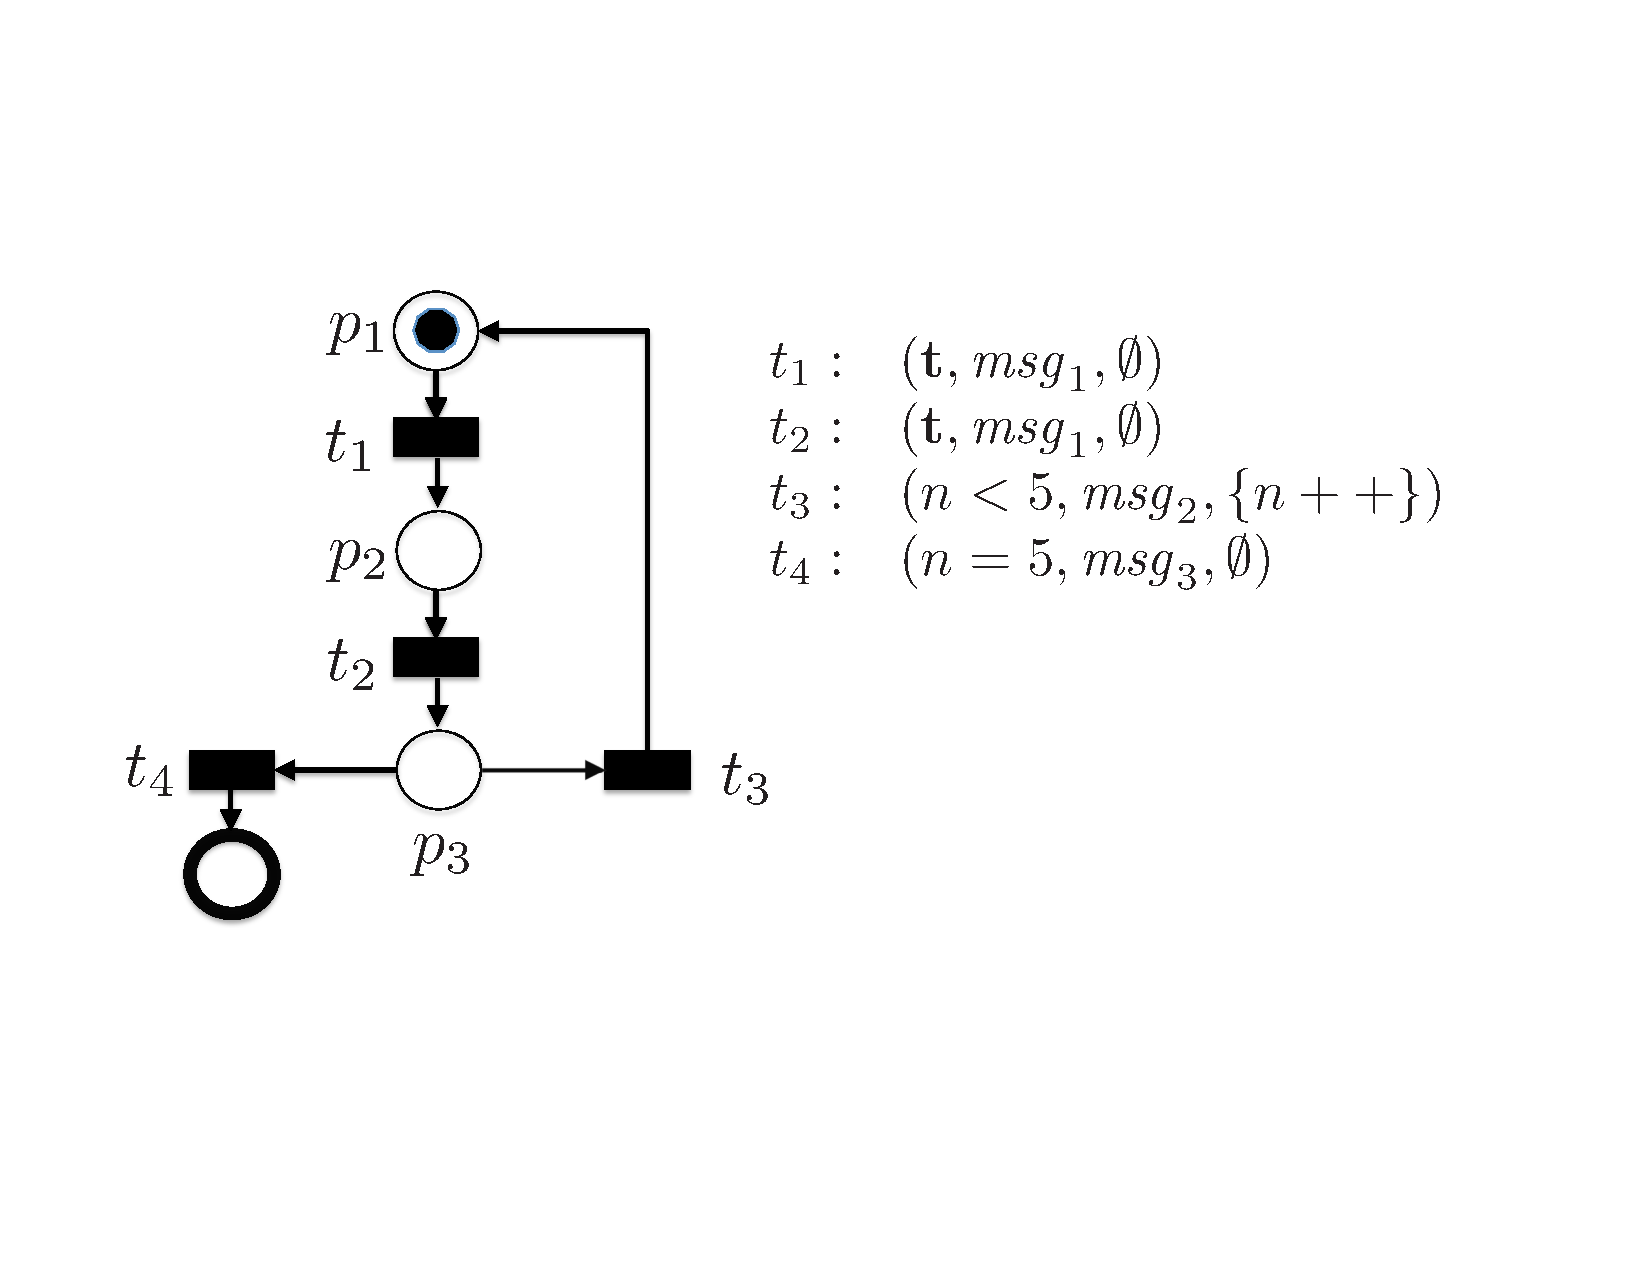
\includegraphics[height=1.6in]{figures/flow-ex-2}
%\caption{Another example of a LPN representing the system flow in Fig.~\ref{fig-flow-ex-1} with a fixed number of message exchanges.}
%\label{fig-flow-ex-2}
%\end{center}
%\end{figure}


%=====




\section{Flow-Directed Trace Interpretation}


%% In a typical validation setting, the system under debug
%% (SUD) is executed in a test environment until it is
%% terminated by the test environment or the system crashes
%% due to a failure.  During the execution, a trace on a
%% small number of observable signals is streamed off the
%% chip for debugging.  Due to the limited observability and
%% inherent non-determinism in today's SoC designs, the
%% observed signal trace is difficult to understand, thus
%% providing limited values for debugging.  In this section,
%% we describe a trace analysis method where the observed
%% signal traces are interpreted at the level of system
%% flows.  In general, the trace analysis can offer
%% debuggers a structured view of communications among the
%% IP blocks during the SUD execution by deriving the types
%% and numbers of system flows activated during SUD
%% executions from the observed signal traces.

%% The trace analysis method consists of two steps:
%% \emph{trace abstraction} and \emph{interpretation}.  The
%% trace abstraction takes a signal trace observed during
%% the execution of the SUD, and abstracts it with respect
%% to information captured in the system flows.  This
%% requires recognizing signal events and mapping the signal
%% events or sequences of the signal events to flow events
%% appeared in system flow specifications.  For example, a
%% data write message may be a single event in a system
%% flow, however, such a flow event maybe implemented in
%% hardware as a sequence of events including a header, a
%% number of data word transfers and a tail.  This
%% abstraction requires a mapping relation from flow events
%% to sequences of signal events, and it is reasonable to
%% assume that this relation is available.

In this section we formalize the trace interpretation
problem in terms of labeled Petri-nets, and discuss our
algorithms to address the problem.  For pedagogical reasons,
here we assume full observability of all hardware signals
involved in the flow events.  In the next section we will
extend the approach to partial observability.

\medskip

\noindent 
{\bf Notations and formalization.}  The set
of system flows is a collection ${\vec{F}}$ of
LPNs.  A {\em flow execution scenario} is defined as a
set $\{(F_{i,j}, s_{i,j})\}$ where $F_{i,j}$ is the
$j$th instance of flow $F_i \in {\vec{F}}$, and $s_{i,j}$ is
a state of $F_{i,j}$.  A flow execution scenario indicates
the set of protocols and the number of instances of a
particular protocol are activated and their corresponding
current states.  Since we assume full observability, we view
an {\em observed trace} $\rho = e_1e_2\ldots e_n$ as a
sequence of events.  Given an observed trace $\rho$, the
goal of trace interpretation is to construct a set of
candidate flow execution scenarios whose execution can
create the sequence of events in $\rho$.  We call such
execution scenarios {\em compliant} with $\rho$.  Let
$\mathit{accept(F_{i,j}, s_{i,j}, e)}$ be a function that
determines if event $e$ can be emitted by $F_{i,j}$ in state
$s_{i,j}$.  Formally, $\mathit{accept(F_{i,j}, s_{i,j}, e)}$
returns $(F_{i,j}, s'_{i,j})$ where $s'_{i,j} = (s_{i,j} - \bullet t)
\cup t\bullet$ if there exists a transition
$t$ in $F_i$ such that $L(t) = e$ and $\bullet t \subseteq
s_{i,j}$.  It returns $\emptyset$ otherwise.

%\medskip

Given an observed trace $\rho$ and the set $\vec{F}$ of LPNs,
Algorithm~\ref{algo:compliance} provides a basic procedure for
computing a set of compliant flow execution scenarios. 
The algorithm operates by keeping track (in variable
$\mathit{Scen}$) of a set of candidate flow execution scenarios
compliant with each prefix of $\rho$.  At each iteration,
for each event $e_h$ in the observed trace, we
update $Scen$ by either extending a member of
$\mathit{scen}$ or initiating a new protocol instance for 
each $scen \in Scen$ with respect to $e_h$ in every possible way.
If $e_h$ cannot be emitted by any existing or new flow instances, 
then we report that the trace is {\tt  inconsistent}, \ie, 
there is no possible interleaving of
the protocol instances from $\vec{F}$ that is compliant with
$\rho$.

\begin{algorithm}[ht]
\DontPrintSemicolon
Create an empty scenario $scen$\;
$\mathit{Scen} = \{scen\}$\;
\ForEach {$h, \; 1 \leq h \leq n $} {
	$\mathit{found} \gets {\tt true}$ \;
	$Scen' = \emptyset$\;
	\ForEach {$scen \in Scen$} {
  		\ForEach {$(F_{i,j}, s_{i,j}) \in \mathit{scen_1}$} {
    		\If {$\mathit{accept}(F_{i,j}, s_{i,j}, e_h) = (F_{i,j}, s'_{i,j})$} {
				Let $scen'$ be a copy of $scen$\;
      		$\mathit{scen'} \gets (\mathit{scen'} - (F_{i,j}, s_{i,j})) \cup (F_{i,j}, s'_{i,j})$\;
      		$\mathit{Scen'} \gets \mathit{scen'} \cup \mathit{Scen'}$\;
      		$\mathit{found} \gets {\tt false}$ \;
    		}
  		}
  		\ForEach {$F_i \in \vec{F}$} {
      	create a new instance $F_{i, j+1}$ \;
      	\If {$\mathit{accept}(F_{i,j+1},\mathit{init}_{i,j+1}, e_h) = (F_{i,j+1}, s'_{i,j+1})$} {
    			Let $scen'$ be a copy of $scen$\;
				$\mathit{scen'} \gets \mathit{scen'} \cup (F_{i,j+1}, s'_{i,j+1})$ \;
				$\mathit{Scen'} \gets \mathit{scen'} \cup \mathit{Scen'}$\;
        		$\mathit{found} \gets {\tt false}$ \;
      	}
    	}
	}
  \If {$\mathit{found} == {\tt true}$} {
    \Return ${\tt Inconsistent}$\;
  }
  $Scen = Scen'$\;
}
\Return $\mathit{Scen}$ \;
\caption{$\textsc{Check-Compliance}(\vec{F}, \, \rho)$}
\label{algo:compliance}
\end{algorithm}

To illustrate the basic idea, consider the system flow in
Fig.~\ref{flow-spec-ex}(b), which we will call $F_1$.
Suppose that the following flow trace is abstracted from an
observed signal trace.
\[
	t_1\;t_2\;t_1\;t_2\;t_3\;t_3\;t_4\;t_5\;t_5\;t_4\ldots
\]  
Here transition names in the LPN are used to represent the 
flow events in the trace.  The first four events results in
the following flow execution scenario
\[
	\{(F_{1,1}, \{p_3\}),~(F_{1,2}, \{p_3\})\}.
\]
For the first event $t_3$, it results in two execution scenarios 
below depending on which flow instance emits $t_3$.
\[
\begin{array}{l}
	\{(F_{1,1}, \{p_4\}),~(F_{1,2}, \{p_3\})\} \\
	\{(F_{1,1}, \{p_3\}),~(F_{1,2}, \{p_4\})\}.
\end{array}
\]
After handing the next event $t_3$, the above two execution scenarios
are reduced to the one as shown below.
\[
	\{(F_{1,1}, \{p_4\}),~(F_{1,2}, \{p_4\})\}.
\]
Using Algorithm~\ref{algo:compliance} to handle the
remaining four events, the following execution scenario is
derived.
\[
	\{(F_{1,1}, \{p_5, p_6\}),~(F_{1,2}, \{p_5, p_6\})\}
\]
%% Given a trace of flow events $\rho = e_1e_2\ldots e_n$, the
%% trace interpretation algorithm starts with an empty set of
%% of flow execution scenario $\mathit{Scen} = \emptyset$.
%% Then, for each $e_h$ where $1 \leq h \leq n$ starting $h=1$,
%% and for each $\mathit{scen} \in \mathit{Scen}$, the
%% following two steps are performed.
%% \begin{description}
%% \item[Step 1]~~For each $(F_{i,j}, s_{i,j}) \in
%%   \mathit{scen}$, if $\mathit{accept}(F_{i,j}, s_{i,j}, e_h)
%%   = (F_{i,j}, s'_{i,j})$, create a new scenario
%%   $\mathit{scen}' = (\mathit{scen} - (F_{i,j}, s_{i,j}))
%%   \cup (F_{i,j}, s'_{i,j})$, which is added into
%%   $\mathit{Scen}'$.

%% \item[Step 2]~~For each $F_i \in \vec{F}$, create a new
%%   instance $F_{i, j+1}$.  If $\mathit{accept}(F_{i,j+1},
%%   \mathit{init}_{i,j+1}, e_h) = (F_{i,j+1}, s'_{i,j+1})$,
%%   create a new scenario $\mathit{scen}' = \mathit{scen} \cup
%%   (F_{i,j+1}, s'_{i,j+1})$, which is added into
%%   $\mathit{Scen}'$.
%% \end{description}

%% After $e_h$ is processed, $Scen = Scen'$, and the above two
%% steps repeat for the next event $e_{h+1}$.

%% If every events in $\rho$ is successfully mapped to some
%% flow instance, this algorithm returns a set of flow
%% execution scenarios such that every flow instance is in its
%% terminal state.  On the other hand, inconsistent events can
%% also be encountered.  An event $e$ is \emph{inconsistent} if
%% for each flow execution scenario $\mathit{scen} \in
%% \mathit{Scen}$, the following two conditions hold.

%% \begin{enumerate}
%% \item For each $(F_{i,j}, s_{i,j}) \in \mathit{scen}$,
%%   $\mathit{accept}(F_{i,j}, s_{i,j}, e_h) = \emptyset$,
%% \item For each $F_i \in \vec{F}$, $\mathit{accept}(F_{i},
%%   \mathit{init}_{i}, e_h) = \emptyset$.
%% \end{enumerate}

%% An inconsistent event is the one produced by SUD execution
%% but cannot be mapped to any flow instances no matter how the
%% trace prior to event $e$ is interpreted.  Inconsistent
%% events indicates possible causes of system failures.

%% Based on the above discussion, the trace interpretation
%% algorithm returns two pieces of information: 1) a set $G$ of
%% flow execution scenarios where every flow instance in every
%% scenario is in its terminal state, 2) a set $B$ of pairs,
%% each of which includes a set of flow execution scenarios and
%% an inconsistent event.  The set $B$ provides valuable
%% information for debuggers to root cause system failures.
%% One of these two sets can empty.  With the full
%% observability, the set $G$ includes a single flow execution
%% scenario derived for a trace.  In reality, it is always the
%% case that the SUD is only partially observable.  Therefore,
%% due to the lack of information for precise interpretation, a
%% set of flow execution scenarios is typically derived for a
%% given trace as the result of the trace analysis.

%% \red{\bf The following illustration may not be needed (from here to the end of this subsection) if seciton IV is kept.  Or we keep the illustration below but remove section IV which uses 3 pages.}

%% To illustrate the basic idea of the trace analysis method, consider the system flow shown in Figure~\ref{fig-flow-ex-1}.  Let $F_1$ denote such flow.  Suppose that a hardware system implements flow $F_1$, and the following trace of flow events is abstracted from an observed signal trace as a result of executing such system.     
%% \[
%% \mathit{msg}_1\;\mathit{msg}_1\;\mathit{msg}_1\;\mathit{msg}_2\;\mathit{msg}_3\;\ldots
%% \]  
%% This trace is interpreted from the first event to the last in order to derive all possible flow execution scenarios.  At the beginning, the first event $\mathit{msg}_1$ is processed.  According to the flow specification $F_1$, we know that one instance of such flow $F_1$, $F_{1,1}$,  is activated by the SUD as $\mathit{accept}(F_{1,1}, init_1, \mathit{msg}_1) = (F_{1,1}, \{p_2\})$ where $\mathit{init} = \{p_1\}$ is the initial state of $F_1$.  As the result, the flow execution scenario after interpreting the first event $\mathit{msg_1}$ is $\{(F_{1,1}, \{p_2\})\}$.  

%% Next, the second $\mathit{msg}_1$ is interpreted on both scenarios   This event could be the result of two possible cases.  In the first case, this event is the result of the continuing execution of $F_{1,1}$ as $\mathit{accept}(F_{1,1}, \{p_2\}, \mathit{msg}_1) = (F_{1,1}, \{p_3\})$.  In the second case, the system may activate another instance of $F_1$, $F_{1,2}$ such that the second event $\mathit{msg_1}$ is a result of executing this new instance.  Therefore, the interpretation of the first two events $\mathit{msg}_1$ leads to two flow execution scenarios as shown below.
%% \[
%% \label{tr-analy-s1}\tag{1}
%% \begin{array}{cl}
%% 1. & \{(F_{1,1}, \{p_3\})\},\\
%% 2. & \{(F_{1,1}, \{p_2\}), (F_{1,2}, \{p_2\})\} 
%% \end{array}
%% \]

%% Now, consider the third $\mathit{msg}_1$ for each of the two scenario derived in~(\ref{tr-analy-s1}).    For the execution scenario~1, $F_{1,1}$ is not able to accept $\mathit{msg}_1$ as it is in state $\{p_3\}$.  On the other hand, this event could be the result of activation of a new flow instance.  Therefore, this execution scenario can be revised accordingly as 
%% \[
%% \label{tr-analy-s2}\tag{2}
%% \{(F_{1,1}, \{p_3\}),(F_{1,2},\{p_2\})\}.
%% \]   
%% For the execution scenario~2, event $\mathit{msg}_1$ could be the result of continuing execution of $F_{1,1}$ or $F_{1,2}$, or it could be a result of activation of a new flow instance.  Therefore,  three new execution scenarios can be derived as shown below for this event.
%% \[
%% \label{tr-analy-s3}\tag{3}
%% \begin{array}{l}
%% \{(F_{1,1}, \{p_3\}), (F_{1,2}, \{p_2\})\},\\
%% \{(F_{1,1}, \{p_2\}), (F_{1,2}, \{p_3\})\}, \\
%% \{(F_{1,1}, \{p_2\}), (F_{1,2}, \{p_2\}), (F_{1,3}, \{p_2\})\}
%% \end{array}
%% \]
%% Since the flow execution scenario in~(\ref{tr-analy-s2}) already exists in~(\ref{tr-analy-s3}), the three flow execution scenarios shown in~(\ref{tr-analy-s3}) is the result from the interpretation of the first three events $\mathit{msg}_1$.

%% The next flow event in the trace $\mathit{msg_2}$ is analyzed for the flow execution scenarios as shown in~(\ref{tr-analy-s3}).   For the first scenario $\{(F_{1,1}, \{p_3\}), (F_{1,2}, \{p_2\})\}$, event $\mathit{msg_2}$ can only be the result from executing $F_{1,1}$ as $\mathit{accept}(F_{1,1}, \{p_3\}, \mathit{msg_2}) = (F_{1,1}, \{p_1\})$.   Based on the same reasoning, this event can only be the result from executing $F_{1,2}$ in the second scenario, and it moves $F_{1,2}$ to a new state $\{p_3\}$ too.  The interesting case is the third scenario where none of the flow instances can allow $\mathit{msg_2}$ to happen.  This is due to the fact that the flow must be in $\{p_3\}$ for $\mathit{msg_2}$ to happen.  This indicates the third system execution scenario is impossible for the prefix of the flow event trace upto $\mathit{msg_2}$, therefore this scenario is ignored from further analysis.  After analyzing event $\mathit{msg_2}$, the updated system execution scenarios are shown below.
%% \[
%% \begin{array}{l}
%% \{(F_{1,1}, \{p_1\}), (F_{1,2}, \{p_2\})\},\ \{(F_{1,1}, \{p2\}), (F_{1,2}, \{p_1\})\}.
%% \end{array}
%% \]

%% The last flow event in the trace is $\mathit{msg}_3$.  Considering the above two possible system executions, neither can allow this event to be produced as none of the flow instances in both system executions is in state $\{p_3\}$.  What this means is that the system does {\em not} implement the flow specification correctly as it produces something not allowed by the specification.  By examining the system executions right before the ``buggy'' event, debuggers may gain more information on when and where the problem might be.  The trace interpretation algorithm adds these two scenarios along with the fifth event $\mathit{msg_3}$ into $B$, and returns it for debuggers to analyze.



%---
\section{Trace Analysis with Partial Observability}


%% In hardware that implements a given system flow
%% specification, a flow event is defined as an event or a
%% sequence of events on a set of signals.  Due to the limited
%% number of pins on the boundary of chips available for
%% observation, only a small fraction of system signals can be
%% observed during debug.  In this section, we discuss how the
%% trace analysis method presented above can be adapted to deal
%% with signal traces of partial observability.

In general, a signal trace of partial observability
corresponds a set of traces of flow events due to the
ambiguous interpretation of signal events.  In the
following, we discuss two cases for trace abstraction on
partial observability: mapping a single signal event to a
flow event or mapping a sequence of signal events to a flow
event.  A signal event is defined as a state on or an
assignment to a set of signals.

Hereafter, the term {\em flow traces} is used to refer to
traces of flow events.  Consider the following example for
the first case.  Suppose that there are three flow events:
$e_1$, $e_2$, and $e_3$, which are implemented in hardware
by the signal events shown in the list below.  We use
Boolean expressions to represent signal events for the
discussion.
\[
\begin{array}{cl}
e_1: & abc\\
e_2: & \bar{a}bc\\
e_3: & a\bar{b}c
\end{array}
\] 
Suppose that only signals $b$ and $c$ are observable, and we
obtain the following trace:
\[
bc\ bc \ \bar{b}c
\]
During trace abstraction, the first two signal events $bc$
can be mapped to $\{e_1, e_2\}$ since $a$ is not observable,
and the last one $b'c$ is mapped to $\{e_3\}$.  Therefore,
this signal trace is abstracted to four flow traces, $\{e_1,
e_2\} \times \{e_1, e_2\} \times \{e_3\}$.

Next, we consider the case where a flow event is mapped from
a sequence of signal events.  Now suppose that two other
flow events are implemented by sequences of signal events as
defined in the list below.
\[
\begin{array}{cl}
e_4: & abc\ \bar{a}bc\\
e_5: & abc\ abc\ abc\ \bar{a}bc\\
\end{array}
\] 
Given an observed trace of the same observability shown below
\[
bc\ bc\ bc \ bc,
\]
it is abstracted to the following flow traces.
\[
e_4e_4,\; \textvisiblespace e_4 \textvisiblespace,\;  e_4 \textvisiblespace \textvisiblespace,\;  \textvisiblespace \textvisiblespace e_4, \; e_5
\] 

where $\textvisiblespace$ denotes signal events that are not
mapped to any flow events.  Note that the above abstraction
leads to three distinct flow traces as the middle three
correspond to the same flow trace.

It is clear from above that a partial trace is viewed as a
set of flow traces, and Algorithm~\ref{algo:compliance} can
be suitably extended to work with flow traces to obtain the
set of candidate flows.  However, applicability of the
algorithm in practice can be gated because the number of
potential flow execution scenarios generated under partial
observability may be enormous.  Note that this is not a
limitation of the algorithm; if the observability of
critical events is poor there simply {\em are} too many flow
execution scenarios compliant with the observed trace.
Nevertheless, we need to address the issue to make trace
interpretation (whether automatic or not) practicable.
There are two potential approaches: (1)~better selection of
post-silicon trace observability, and (2)~use of system
insights during validation.  Trace signal selection itself
is an important and orthogonal topic~\cite{nicolici,basu},
and a detailed discussion of it is out of scope of this
paper.  However, we briefly describe how the debuggers'
insights of a system's architecture can help to address the
complexity issue in the trace interpretation.


\subsection{Interactive Trace Interpretation}

Post-silicon validation is performed by debuggers with deep
knowledge about the system's architecture and
microarchitecture, and the test environment.  Two key
insights are (1) the maximal number of instances of a flow
activated in the test environment, and (2)~the mutual
relationship between two flows.  For example, the test
environment may not permit multiple instances of firmware
authentication to operate concurrently, or a flow involving
audio and Web browsing to initiate until the flows
participating in boot are completed.  Our framework permits
incorporating such insights as constraints in trace
analysis; flow execution scenarios that violate these
constraints are ignored.  \textcolor{red}{These insights can lead to two advantages.
First, they help to reduce the potentially large number of partial
scenarios generated during the trace interpretation step, thus making 
the analysis more efficient.  Second, they permit the debugger
to quickly filter out uninteresting combinations of flows and focus on interesting
interleavings.}

This approach can be flexible in that it allows a debugger
to analyze the observed traces in a trail-and-error manner
if the precise knowledge of the system (micro-)architecture
is hard to come by.  For instance, the debugger might
initially make a very restricted assumption on how the SUD
executes a flow specification, and these assumptions can
potentially lead to an empty set of flow execution
scenarios.  Depending on which of these assumptions
triggered during the trace interpretation step, the debugger
can study these assumptions more carefully, and relax some
or all of them for the next run of analysis.  This iteration
can be repeated as many times as necessary until some
results deemed meaningful are produced.

%% Alternatively, if all derived execution scenarios seem to be
%% plausible, the implication that a debugger may draw from
%% this result is that the failure may be independent of the
%% flows being observed.  Therefore, the testing environment
%% can be adjusted in order for a different part or different
%% behavior of the SUD to be observed.  This idea, closely
%% related to trace signal selection, is critical for
%% post-silicon validation, and a detailed discussion can only
%% be presented in a separate paper.


  
%%-- Case study I
%%=====
\section{Case Study}

The proof concept of the proposed trace analysis method is demonstrated on a transaction level model of a simple SoC design with two CPU cores, memory, and a peripheral device connected by an interconnect as shown in Fig.~\ref{fig-SoC-ex}.  Since the analysis method presented in this paper is communication centric, the detailed computations of these blocks are not modeled.  Instead, the modeling is focused on how they participate in flows for different system level use cases.

\begin{figure}[tb]
\begin{center}
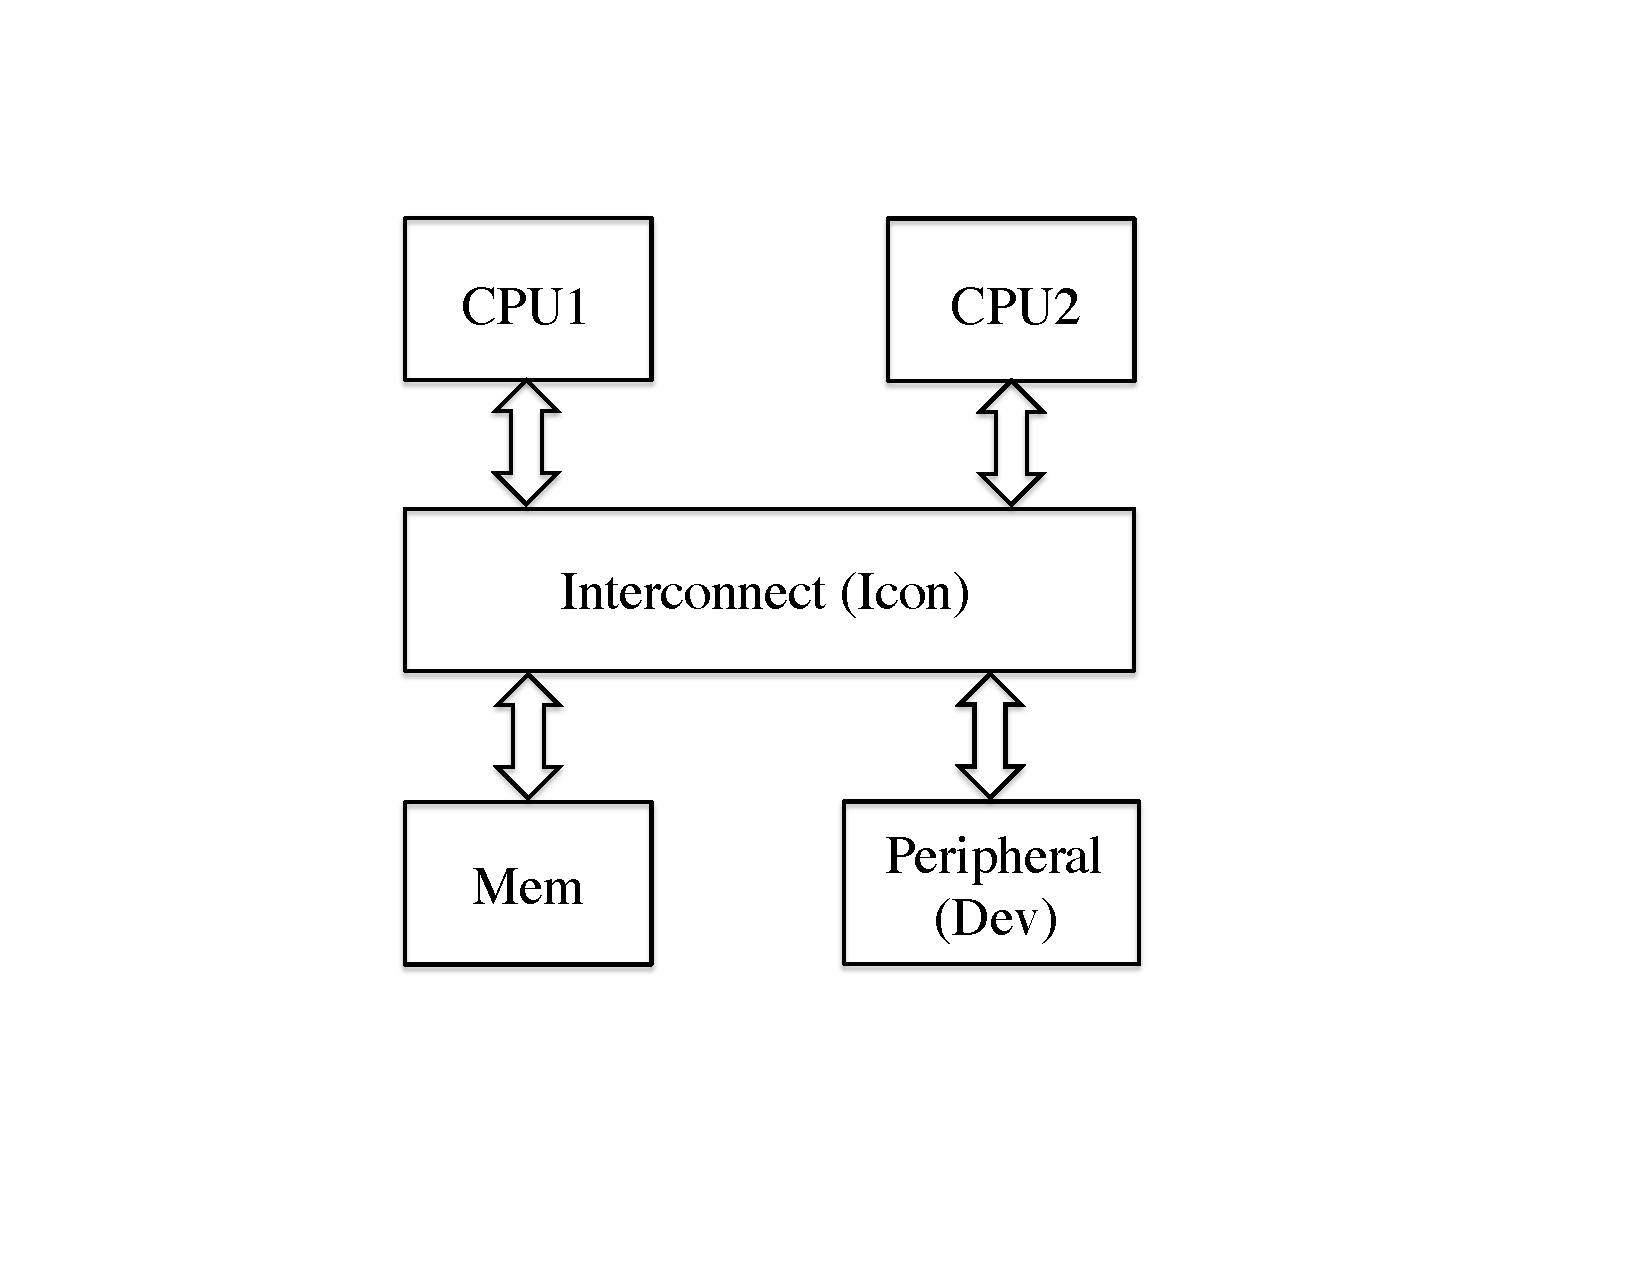
\includegraphics[width=2in]{figures/simple-ex}
\caption{A simple SoC example.}
\label{fig-SoC-ex}
\end{center}
\end{figure}


\subsection{Flow Specification}

In this case study, four system flows are implemented in the simple SoC model. They include cache coherent memory access operations and a memory-mapped peripheral read operation initiated from the CPUs, a message signaled interrupt operation initiated from the peripheral device.  These flow specifications capture how messages are exchanged for different use cases.  In this model, a message is defined with the following format, $(\mbox{Src}, \mbox{Dest}, \mathit{Cmd}, \mathit{Addr})$, where Src and Dest refer to the source and destination components of messages, $\mathit{Cmd}$ refers to the operations that the destination component should perform, and $\mathit{Addr}$ refers to memory addresses where $\mathit{Cmd}$ applies.  $\mathit{Cmd}$ can be memory accesses or not.  If it is not, then the $\mathit{Addr}$ field of messages is ignored.  In this case study, memory mapped IO mechanism is used.  Furthermore, detailed memory addresses are not modeled. Instead, the address space is partitioned to main memory addresses and peripheral addresses.  In messages, the $\mathit{Addr}$ field is replaced with either $M$ representing a memory address or $P$ representing an address to a peripheral device.  

The LPN as shown in Fig.~\ref{fig-cpu-write} specifies a system flow where {CPU2} initiates a memory write operation.   In this flow, CPU2 initiates a memory write request followed by a data valid message to the interconnect.  The data valid messages are used to model availability or validity of data for transfer.  Concurrently, the interconnect inquiries CPU1 if it holds a more updated version of the data by sending a memory write message $\mathit{msg_2}$.   CPU1 generates one of two possible responses.  If CPU1 holds the more updated data in its cache in the same memory space that CPU2 intends to write, a cache hit message $\mathit{msg_4}$ followed by $\mathit{msg_6}$ are sent to the interconnect.  Otherwise, CPU1 sends a cache miss message $\mathit{msg_5}$.  After getting the response from CPU1, Interconnect sends a write request to the memory unit.  This flow is symmetric for CPU1.

\begin{figure}[tb]
\begin{center}
\resizebox{2.8in}{!}{
\begin{tikzpicture}[node distance=3cm, auto,>=latex', thick]
\tikzset{rectbox/.style={rectangle, draw, align=flush center,thick, minimum size = 6mm}}
\tikzset{circ/.style={circle, draw,thick}}
\tikzset{terminal/.style={circle, draw,line width=.8mm}}
\tikzset{weight3/.style={line width=.3mm}}
	% Nodes:
	\node[circ]		(p1) 		at (0,0) {$p_1$};
	\node[rectbox]	(msg1)	at	($(p1) + (0,-1.1)$) {$msg_1$};
	\node[circ] 	(p2) 		at ($(msg1) + (-3,0)$) {$p_2$};
	\node[circ] 	(p3) 		at ($(msg1) + (3,0)$) {$p_3$};
	\node[rectbox]	(msg2)	at	($(p2) + (0,-1.1)$) {$msg_2$};
	\node[rectbox]	(msg3)	at	($(p3) + (0,-1.5)$) {$msg_3$};
	\node[circ] 	(p4) 		at ($(msg2) + (0,-1.1)$) {$p_4$};
	\node[rectbox]	(msg4)	at	($(p4) + (0,-1.1)$) {$msg_4$};
	\node[rectbox]	(msg5)	at	($(p4) + (3,0)$) {$msg_5$};
	\node[circ] 	(p6) 		at ($(msg4) + (0,-1.1)$) {$p_6$};
	\node[circ] 	(p5) 		at ($(msg3) + (0,-1.4)$) {$p_5$};
	\node[rectbox,rotate=90]	(msg6)	at	($(p6) + (1.5,0)$) {$msg_6$};
	\node[circ] 	(p7) 		at ($(msg6) + (1.5,0)$) {$p_7$};
	\node[rectbox]	(msg7)	at	($(p5) + (0,-1.5)$) {$msg_7$};
	\node[terminal]	(p8)	at	($(msg7) + (2,0)$) {$p_8$};
	% Edges
	\draw[->,weight3]	(p1) -- (msg1);
	\draw[->,weight3]	(msg1) -- (p2);
	\draw[->,weight3]	(msg1) -- (p3);
	\draw[->,weight3]	(p2) -- (msg2);
	\draw[->,weight3]	(msg2) -- (p4);
	\draw[->,weight3]	(p4) -- (msg4);
	\draw[->,weight3]	(p4) -- (msg5);
	\draw[->,weight3]	(msg4) -- (p6);
	\draw[->,weight3]	(p6) -- (msg6);
	\draw[->,weight3]	(msg6) -- (p7);
	\draw[->,weight3]	(p7) -- (msg7);
	\draw[->,weight3]	(msg7) -- (p8);
	\draw[->,weight3]	(msg5) -- (p7);
	\draw[->,weight3]	(p3) -- (msg3);
	\draw[->,weight3]	(msg3) -- (p5);
	\draw[->,weight3]	(p5) -- (msg7);
	
	\node[]	(msg-def)	at	($(p1) + (0,-8.5)$) {
	\begin{minipage}{3in}
	Definition of the messages:
\[
\begin{array}{clllll}
msg_1: & (\mbox{CPU2},	& \mbox{Icon},		& \mathit{Wr}, 	& M) \\
msg_2: & (\mbox{Icon},	& \mbox{CPU1}, 	& \mathit{Wr},			& M) \\
msg_3: & (\mbox{CPU2},	& \mbox{Icon}, 	& \mathit{DVal},	& -) \\
msg_4: & (\mbox{CPU1},	& \mbox{Icon}, 	& \mathit{Hit},	& -) \\
msg_5: & (\mbox{CPU1},	& \mbox{Icon}, 	& \mathit{Miss},	& -) \\
msg_6: & (\mbox{CPU1},	& \mbox{Icon}, 	& \mathit{DVal},	& -) \\
msg_7: & (\mbox{Icon},	& \mbox{Mem}, 		& \mathit{Wr},			& M) \\
\end{array}
\]
\end{minipage}
		};
\end{tikzpicture}
}
\caption{Flow specification ($F_1$) of a cache coherent write operation initiated from \texttt{CPU2}.}
\label{fig-cpu-write}
\end{center}
\end{figure}


The LPN specification as shown in Fig.~\ref{fig-cpu-read} captures the system flow where CPU2 initiates a memory read operation.  Basically, CPU2 sends a memory read message to Interconnect, which then generates two concurrent threads, one checks if CPU1 has the more updated data in the memory space for the read operation, and the other thread to get data from the memory.  Once Interconnect gets both responses from CPU1 and memory, it synchronizes the responses, and writes the correct data to the CPU2's cache and memory in parallel.  Again, this specification is symmetric for CPU1.


\begin{figure}[htbp]
\begin{center}
\resizebox{3.2in}{!}{
\begin{tikzpicture}[node distance=3cm, auto,>=latex', thick]
\tikzset{rectbox/.style={rectangle, draw, align=flush center,thick, minimum size = 6mm}}
\tikzset{circ/.style={circle, draw,thick}}
\tikzset{terminal/.style={circle, draw,line width=.8mm}}
\tikzset{weight3/.style={line width=.3mm}}
	% Nodes:
	\node[circ]		(p1) 		at (0,0) {$p_1$};
	\node[rectbox]	(msg1)	at	($(p1) + (0,-1.1)$) {$msg_1$};
	\node[circ] 	(p2) 		at ($(msg1) + (-3,0)$) {$p_2$};
	\node[circ] 	(p3) 		at ($(msg1) + (2,0)$) {$p_3$};
	\node[rectbox]	(msg2)	at	($(p2) + (0,-1.1)$) {$msg_2$};
	\node[rectbox]	(msg3)	at	($(p3) + (2,0)$) {$msg_3$};
	\node[circ] 	(p4) 		at ($(msg2) + (0,-1.1)$) {$p_4$};
	\node[rectbox]	(msg4)	at	($(p4) + (0,-1.1)$) {$msg_4$};
	\node[rectbox]	(msg5)	at	($(p4) + (3,0)$) {$msg_5$};
	\node[circ] 	(p6) 		at ($(msg4) + (0,-1.1)$) {$p_6$};
	\node[circ] 	(p5) 		at ($(msg3) + (0,-1.1)$) {$p_5$};
	\node[rectbox,rotate=90]	(msg6)	at	($(p6) + (1.5,0)$) {$msg_6$};
	\node[circ] 	(p7) 		at ($(msg6) + (1.5,0)$) {$p_7$};
	\node[rectbox]	(msg7)	at	($(p5) + (0,-1.1)$) {$msg_7$};
	\node[circ]	(p8)	at	($(msg7) + (0,-1.1)$) {$p_8$};
	\node[rectbox]	(msg8)	at	($(p8) + (0,-1.1)$) {$msg_8$};
	\node[circ]	(p9)	at	($(msg8) + (-1.5,-1.1)$) {$p_9$};
	\node[circ]	(p10)	at	($(msg8) + (1.5,-1.1)$) {$p_{10}$};
	\node[rectbox]	(msg9)	at	($(p9) + (0,-1.1)$) {$msg_9$};
	\node[rectbox]	(msg10)	at	($(p10) + (0,-1.1)$) {$msg_{10}$};
	\node[terminal]	(p11)	at	($(msg9) + (0,-1.1)$) {$p_{11}$};
	\node[terminal]	(p12)	at	($(msg10) + (0,-1.1)$) {$p_{12}$};

	% Edges
	\draw[->,weight3]	(p1) -- (msg1);
	\draw[->,weight3]	(msg1) -- (p2);
	\draw[->,weight3]	(msg1) -- (p3);
	\draw[->,weight3]	(p2) -- (msg2);
	\draw[->,weight3]	(msg2) -- (p4);
	\draw[->,weight3]	(p4) -- (msg4);
	\draw[->,weight3]	(p4) -- (msg5);
	\draw[->,weight3]	(msg4) -- (p6);
	\draw[->,weight3]	(p6) -- (msg6);
	\draw[->,weight3]	(msg6) -- (p7);
	\draw[->,weight3]	(p7) -- (msg8);
	\draw[->,weight3]	(msg7) -- (p8);
	\draw[->,weight3]	(msg5) -- (p7);
	\draw[->,weight3]	(p3) -- (msg3);
	\draw[->,weight3]	(msg3) -- (p5);
	\draw[->,weight3]	(p5) -- (msg7);
	\draw[->,weight3]	(p8) -- (msg8);
	\draw[->,weight3]	(msg8) -- (p9);
	\draw[->,weight3]	(msg8) -- (p10);
	\draw[->,weight3]	(p9)  -- (msg9);
	\draw[->,weight3]	(p10)  -- (msg10);
	\draw[->,weight3]	(msg9) -- (p11);
	\draw[->,weight3]	(msg10) -- (p12);
	
	\node[]	(msg-def)	at	($(p1) + (-2.7,-10)$) {
	\begin{minipage}{2in}
	Definition of the messages:
\[
\begin{array}{clllll}
msg_1: & (\mbox{CPU2},	& \mbox{Icon},		& \mathit{Rd}, 		& M) \\
msg_2: & (\mbox{Icon},	& \mbox{CPU1}, 	& \mathit{Rd},	& M) \\
msg_3: & (\mbox{Icon},	& \mbox{Mem}, 		& \mathit{Rd},			& M) \\
msg_4: & (\mbox{CPU1},	& \mbox{Icon}, 	& \mathit{Hit},	& -) \\
msg_5: & (\mbox{CPU1},	& \mbox{Icon}, 	& \mathit{Miss},& -) \\
msg_6: & (\mbox{CPU1},	& \mbox{Icon}, 	& \mathit{DVal},	& -) \\
msg_7: & (\mbox{Mem},		& \mbox{Icon}, & \mathit{DVal},			& -) \\
msg_8: & (-,		& -, 		& -,				& -) \\
msg_9: & (\mbox{Icon},	& \mbox{Mem}, 		& \mathit{Wr},			& M) \\
msg_{10}: & (\mbox{Icon},	& \mbox{CPU2}, 		& \mathit{Wr},			& M) \\
\end{array}
\]
\end{minipage}
		};

\end{tikzpicture}
}
\caption{Flow specification ($F_2$) of a cache coherent read operation from CPU2.}
\label{fig-cpu-read}
\end{center}
\end{figure}


The LPN specification as shown in Fig.~\ref{fig-peri-read} captures a system flow for CPU initiated memory mapped peripheral read operations.  When CPU2 tries to read the peripheral device (device hereafter), a read message with address $P$ is sent to Interconnect, which then sends this message to CPU1 and the device simultaneously.  When CPU1 sees this message, it responds with a cache miss message as the address $P$ points to the device.  At the meantime, the device responds with a data valid message indicating the availability of the requested data.  Finally, Interconnect synchronizes the both responses, and sends a data valid message back to CPU2.   This specification is also symmetric for CPU1.

\begin{figure}[tb]
\begin{center}
\resizebox{3.2in}{!}{
\begin{tikzpicture}[node distance=3cm, auto,>=latex', thick]
\tikzset{rectbox/.style={rectangle, draw, align=flush center,thick, minimum size = 6mm}}
\tikzset{circ/.style={circle, draw,thick}}
\tikzset{terminal/.style={circle, draw,line width=.8mm}}
\tikzset{weight3/.style={line width=.3mm}}
	% Nodes:
	\node[circ]		(p1) 		at (0,0) {$p_1$};
	\node[rectbox]	(msg1)	at	($(p1) + (0,-1.1)$) {$msg_1$};
	\node[circ] 	(p2) 		at ($(msg1) + (-1.5,0)$) {$p_2$};
	\node[circ] 	(p3) 		at ($(msg1) + (1.5,0)$) {$p_3$};
	\node[rectbox]	(msg2)	at	($(p2) + (-1.5,0)$) {$msg_2$};
	\node[rectbox]	(msg4)	at	($(p3) + (1.5,0)$) {$msg_4$};
	\node[circ] 	(p4) 		at ($(msg2) + (-1.5,0)$) {$p_4$};
	\node[rectbox]	(msg3)	at	($(p4) + (0,-1.2)$) {$msg_3$};
	\node[circ] 	(p6) 		at ($(msg3) + (0,-1.2)$) {$p_6$};
	\node[circ] 	(p5) 		at ($(msg4) + (1.5,0)$) {$p_5$};
	\node[rectbox]	(msg5)	at	($(p5) + (0,-1.2)$) {$msg_5$};
	\node[circ]	(p7)	at	($(msg5) + (0,-1.2)$) {$p_7$};
	\node[rectbox]	(msg6)	at	($(p6) + (4.5,0)$) {$msg_6$};
	\node[terminal]	(p8)	at	($(msg6) + (0,-1.2)$) {$p_8$};

	% Edges
	\draw[->,weight3]	(p1) -- (msg1);
	\draw[->,weight3]	(msg1) -- (p2);
	\draw[->,weight3]	(msg1) -- (p3);
	\draw[->,weight3]	(p2) -- (msg2);
	\draw[->,weight3]	(msg2) -- (p4);
	\draw[->,weight3]	(p4) -- (msg3);
	\draw[->,weight3]	(msg3) -- (p6);
	\draw[->,weight3]	(p6) -- (msg6);
	\draw[->,weight3]	(msg6) -- (p8);
	\draw[->,weight3]	(p3) -- (msg4);
	\draw[->,weight3]	(msg4) -- (p5);
	\draw[->,weight3]	(p5) -- (msg5);
	\draw[->,weight3]	(msg5) -- (p7);
	\draw[->,weight3]	(p7) -- (msg6);
	\draw[->,weight3]	(msg6) -- (p8);
	
		\node[]	(msg-def)	at	($(p8) + (0,-2.5)$) {
	\begin{minipage}{3in}
	Definition of the messages:
\[
\begin{array}{clllll}
msg_1: & (\mbox{CPU2},	& \mbox{Icon},		& Rd, 	& P) \\
msg_2: & (\mbox{Icon},	& \mbox{CPU1}, 	& Rd,		& P) \\
msg_3: & (\mbox{CPU1},	& \mbox{Icon}, 	& Miss,			& -) \\
msg_4: & (\mbox{Icon},	& \mbox{Dev}, 	& Rd,	& P) \\
msg_5: & (\mbox{Dev},	& \mbox{Icon}, 	& Dval,	& -) \\
msg_6: & (\mbox{Icon},	& \mbox{CPU2}, 	& Dval,	& -) \\\end{array}
\]
\end{minipage}
		};
\end{tikzpicture}
}
\caption{Flow specification ($F_3$) of a read access to peripheral device from CPU2.}
\label{fig-peri-read}
\end{center}
\end{figure}


The last LPN specification as shown in Fig.~\ref{fig-msi} captures how interrupts from the device are handled.  In this case study, all interrupts are directed to CPU1.  When the device triggers an interrupts, it sends a message with $\mathit{Intr}$ in the command field.  Then, Interconnect notifies CPU1 by sending a message with $\mathit{MSI}$ and $I$ in the command and address fields, respectively, where $I$ is the symbol referring to the entry points to interrupt service routines.   CPU1 responds with a cache miss message as the receipt of the interrupt.   


\begin{figure}[htbp]
\begin{center}
\resizebox{3.5in}{!}{
\begin{tikzpicture}[node distance=3cm, auto,>=latex', thick]
\tikzset{rectbox/.style={rectangle, draw, align=flush center,thick, minimum size = 6mm}}
\tikzset{circ/.style={circle, draw,thick}}
\tikzset{terminal/.style={circle, draw,line width=.8mm}}
\tikzset{weight3/.style={line width=.3mm}}
	% Nodes:
	\node[circ]		(p1) 		at (0,0) {$p_1$};
	\node[rectbox]	(msg1)	at	($(p1) + (1.5, 0)$) {$msg_1$};
	\node[circ] 	(p2) 		at ($(msg1) + (1.5, 0)$) {$p_2$};
	\node[rectbox]	(msg2)	at	($(p2) + (1.5,0)$) {$msg_2$};
	\node[circ] 	(p3) 		at ($(msg2) + (1.5, 0)$) {$p_3$};
	\node[rectbox]	(msg3)	at	($(p3) + (1.5, 0)$) {$msg_3$};
	\node[terminal] 	(p4) 		at ($(msg3) + (1.5,0)$) {$p_4$};
	
	% Edges
	\draw[->,weight3]	(p1) -- (msg1);
	\draw[->,weight3]	(msg1) -- (p2);
	\draw[->,weight3]	(p2) -- (msg2);
	\draw[->,weight3]	(msg2) -- (p3);
	\draw[->,weight3]	(p3) -- (msg3);
	\draw[->,weight3]	(msg3) -- (p4);
	
	
\node[]	(msg-def)	at	($(msg2) + (0,-2)$) {
	\begin{minipage}{3in}
	Definition of the messages:
\[
\begin{array}{clllll}
msg_1: & (\mbox{Dev},	& \mbox{Icon},		& \mathit{Intr}, 	& -) \\
msg_2: & (\mbox{Icon},	& \mbox{CPU1}, 	& \mathit{MSI},	& I) \\
msg_3: & (\mbox{CPU1},	& \mbox{Icon}, 	& \mathit{Miss},	& -) \\
\end{array}
\]
\end{minipage}
		};
\end{tikzpicture}
}
\caption{Flow specification ($F_4$) of handling interrupts from the peripheral device.}
\label{fig-msi}
\end{center}
\end{figure}


%
%
\subsection{Results and Discussions}
%
%
The transaction level model of the simple system implementing the four flow specifications shown in the previous section is described in SystemC.  Each component is described as a SystemC module, which may include a number of threads to model concurrency.  The entire model is concurrent and operates in asynchronous mode.  

When testing this model, both CPUs and the peripheral device are set up as flow instance generators.  They randomly generate the first message in a corresponding flow specification to start a flow instance, and react to incoming messages by generating new messages as defined in the flow specification.  In the model, monitors are embedded to observe the messages generated by each component.  When a message is observed, it is written to an output trace file for analysis.   

Even though this example is conceptually simple, getting the model to correctly implement the flow specifications is not straightforward.  On the other hand, results from the trace analysis greatly help the debugging process by providing information to locate problems quickly.  For example, in an early version of the model, the trace shown in Table~\ref{table-trace} is observed.  
\begin{table*}
\caption{An observed trace of messages for trace analysis.}
\label{table-trace}
\begin{center}
\begin{tabular}{llll}
1~~(CPU2, Icon, Rd, M) & 2~~(Icon, CPU1, Rd, M) & 3~~(Icon, Mem, Rd, M) & 4~~(Mem,  Icon, DVal, -) \\
5~~(CPU1, Icon, Hit, -) & 6~~(CPU1, Icon, DVal, -) & 7~~(Icon, CPU2, Wr, M) & 8~~(Icon, Mem, Wr, M) \\
9~~(CPU2, Icon, Rd, M) & 10~(Icon, CPU1, Rd, M) & 11~(Icon, Mem, Rd, M) & 12~(CPU2, Icon, Rd, P) \\
13~(Icon, CPU1, Rd, P) & 14~(CPU1, Icon, Miss, -) & 15~(Icon, Dev, Rd, P) & 16~(CPU1, Icon, DVal, -) \\
\end{tabular}
\end{center}
\end{table*}
The trace analysis finds out that messages~$1-8$ in the trace are the results of execution of an instance of flow $F_2$ as shown, and the flow execution scenario is $\{(F_{2,1}, \{p_{11}, p_{12}\})\}$.  Messages~$9-11$ are analyzed as the results of executing another instance of flow $F_2$, message~$12-13$ as the results of executing an instance of flow $F_3$ as shown in Fig.~\ref{fig-peri-read}.  The flow execution scenario after the first thirteen messages in the trace is 
\[
\{(F_{2,1}, \{p_{11}, p_{12}\}), (F_{2,2}, \{p_4, p_5\}), (F_{3,1}, \{p_4, p_3\})\}.
\]  
Message~$14$ can be  the result from executing $F_{2,2}$ or $F_{3,1}$, therefore it leads to two following flow execution scenarios:
\begin{equation}
\{(F_{2,1}, \{p_{11}, p_{12}\}), (F_{2,2}, \{p_7, p_5\}), (F_{3,1}, \{p_4, p_3\})\}
\end{equation}
\begin{equation}
\{(F_{2,1}, \{p_{11}, p_{12}\}), (F_{2,2}, \{p_4, p_5\}), (F_{3,1}, \{p_6, p_3\})\}
\end{equation}
In either scenario, after mapping message~$15$ to flow $F_{3,1}$, message~$16$ cannot be mapped to any existing flow instance or to a new flow instance.  From this inconsistent message, we know that it is generated by CPU1.  In scenario~(1), CPU1 is in the state after generating the message reporting a cache miss.  In this case, the DataValid message should not generated.  In scenario~(2), CPU1 is in the state before generating the message reporting either a cache hit or miss, and again the DataValid message should not generated.   This inconsistent message helps to locate a bug in the CPU1 model where a DataValid message is generated after either a cache hit or miss message is generated.  After fixing this bug,  in a few more iterations of analysis and debugging, the trace analysis can eventually extract all initiated flow instances in the model, all in their terminal states, thus showing that the model implements the four flows correctly.


In the second experiment, partial observability is taken into account during the trace analysis with the assumption that the command $\mathit{Wr}$ and $\mathit{Rd}$ and addresses $M$ and $P$ are indistinguishable due to the lack of observability.  This partial observability is simulated with a modification to the monitors such that in each observed message, command $\mathit{Wr}$ or $\mathit{Rd}$ is replaced with $(\mathit{Wr},\mathit{Rd})$ and address $M$ or $P$ is replaced with $(M,P)$.  The version of the model generating the trace shown in Table~\ref{table-trace} is reused with the modified the monitors, and the generated trace with the simulated partial observability is shown in Table~\ref{table-trace-2}.  Similarly, only the first sixteen messages are shown. 
\begin{table*}
\caption{A trace of messages with partial observability for trace analysis.}
\label{table-trace-2}
\begin{center}
\resizebox{7.3in}{!}{
\begin{tabular}{llll}
1~~(CPU2, Icon, (Wr, Rd), (M, P)) & 2~~(Icon, CPU1, (Wr, Rd), (M, P)) & 3~~(Icon, Mem, (Wr, Rd), (M, P)) & 4~~(Mem,  Icon, DVal, -) \\
5~~(CPU1, Icon, (Hit, Miss), -) & 6~~(CPU1, Icon, DVal, -) & 7~~(Icon, CPU2, (Wr, Rd), (M, P)) & 8~~(Icon, Mem, (Wr, Rd), (M, P)) \\
9~~(CPU2, Icon, (Wr, Rd), (M, P)) & 10~(Icon, CPU1, (Wr, Rd), (M, P)) & 11~(Icon, Mem, (Wr, Rd), (M, P)) & 12~(CPU2, Icon, (Wr, Rd), (M, P)) \\
13~(Icon, CPU1, (Wr, Rd), (M, P)) & 14~(CPU1, Icon, (Hit, Miss), -) & 15~(Icon, Dev, (Wr, Rd), (M, P)) & 16~(CPU1, Icon, DVal, -) \\
\end{tabular}
}
\end{center}
\end{table*}

Each message in the trace with partial observability is referred to as an {\em super} message to distinguish it from the messages of full observability.  The traces of super messages are referred to as {\em super} traces.  For example, the first super message in the trace from Table~\ref{table-trace-2}, $\mbox{(CPU2, Icon, (Wr, Rd), (M, P))}$, corresponds to four distinct messages:
$\mbox{(CPU2, Icon, Wr, M)}$, $\mbox{(CPU2, Icon, Wr, P)}$, $\mbox{(CPU2, Icon, Rd, M)}$, and $\mbox{(CPU2, Icon, Rd, P)}$.  Some of these messages do not exist in the flow specification, and are ignored during the trace analysis.   In the above example, message $\mbox{(CPU2, Icon, Wr, P)}$ is ignored.

%Each super trace represents a set of traces, each of which is interpreted to derive a set of flow execution scenarios.  These flow execution scenarios can show different inconsistent messages.  For example, the particular trace of the super trace shown in Table~\ref{table-trace-2} below
%\[
%\mbox{1 (CPU2, Icon, Wr, M), 2~(Icon, CPU1, Rd, M)}, \ldots
%\]
%leads to the following flow execution scenario $\{(F_{1,1}, \langle p_2,p_3\rangle)\}$ showing that the second message is inconsistent.  In addition, this super trace also represents a trace as shown in Table~\ref{table-trace} that leads to a real bug in the model as discussed above.  It is also possible in some situation that a super trace may represent a trace with no inconsistent messages.  Therefore, the trace analysis on a super trace can result in a number of flow execution scenarios revealing different problems or no problem.  This ambiguity is caused by the partial observability.  

Each super trace represents a set of traces, each of which is interpreted to derive a set of flow execution scenarios.
Due to the partial observability, the number of traces represented by a super trace can become very large. For example, the super trace shown in Table~\ref{table-trace-2} represents about twelve thousand possible traces for that short sequence of messages.  The trace analysis algorithm returns the set of flow execution scenarios for each trace for examination, and a very large number of possible flow execution scenarios can be generated.  The large number of possible flow execution scenarios not only produces too much information that can overwhelm system validators, but also degrades the performance of the trace analysis algorithm by consuming too much memory.  As indicated above,  the validators' insights on the SUD can be utilized to trim the possibilities.  For example, if the validator knows that no flow $F_1$ in Fig.~\ref{fig-cpu-write} is activated in the testing environment, this insight helps to eliminate all flow execution scenarios that include instances of $F_1$ by interpreting message~$\#1$ as either $\mbox{(CPU2, Icon, Rd, M)}$ or $\mbox{(CPU2, Icon, Rd, P)}$.  Consider another insight such that a new instance of flow $F_2$ as in Fig.~\ref{fig-cpu-read} can be initiated only after the completion of the previous instance of $F_2$.  If an instant of $F_2$ is assumed to be initiated by the super message $\#9~\mbox{(CPU2, Icon, (Wr, Rd), (M, P))}$ by interpreting it to $\mbox{(CPU2, Icon, Rd, M)}$ during the trace analysis, the super message~$\#12$ can only be interpreted to $\mbox{(CPU2, Icon, Wr, M)}$ or $\mbox{(CPU2, Icon, Rd, P)}$ as the instance of $F_2$ initiated by the super message $\#9$ has not been completed yet at this point.   According to the above discussion, the validators' insights help restrict how super messages are interpreted, thus reducing the number of flow execution scenarios that can be generated.
At the end of the analysis, all possible flow execution scenarios are returned to system validators for examination. 



%
%--
%
\section{Case Study}

%% The proposed method is demonstrated on a transaction level
%% model of a simple SoC design with CPU core, memory, and a
%% peripheral device connected by a highly concurrent
%% interconnect in SystemC.  Since the proposed method is
%% communication centric, the detailed computations of these
%% blocks are not modeled.  Instead, the modeling is focused on
%% how they participate in system level protocols.  This simple
%% case study shows that the proposed method is capable of
%% providing useful information to help reveal and locate
%% various bugs in the SystemC model, thus making the debugging
%% more efficient.  Once a bug-free model is available, the
%% trace analysis method can correctly derive the instances of
%% system flows activated by various components in the design
%% from the observed traces.  More details about the design
%% model and system flows implemented by the design model will
%% be provided in a supplement document stored online.


\begin{figure} 
\centerline{
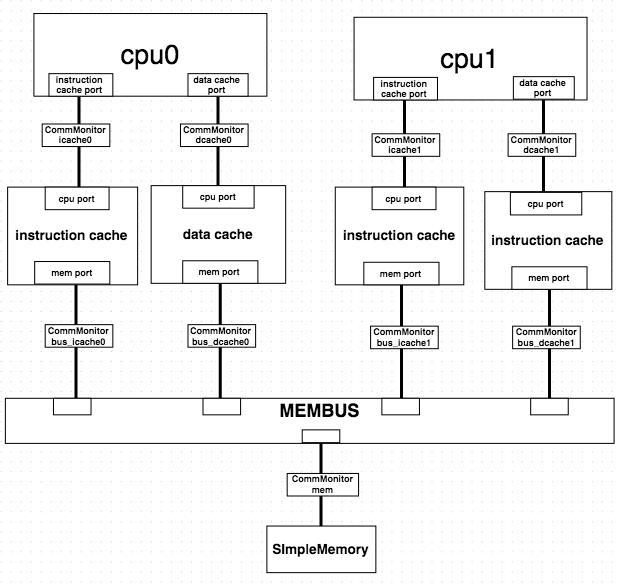
\includegraphics[width=3in]{figures/Fig4.png}}
\caption{SoC platform structure.}
\label{SoC}
\end{figure}

In order to find out the efficiency of the trace analysis
method for more realistic examples, in the case study
described in this section, a more detailed transaction level
model of a SoC is constructed within the GEM5
environment~\cite{Binkert2011}.  This SoC model, as shown in Fig.~\ref{SoC},
consists of
two ARM Cortex-A9 cores, each of which contains two separate
16KB data and instruction caches.  The caches are connected
to a 1GB memory through a memory bus model. 

In this model, components communicate with each other by
sending and receiving various request and response messages.
In order to observe and trace communications occurring
inside this model during execution, monitors are attached to
links connecting the components. These monitors record the
messages flowing through the links they are attached to, and
store them into output trace files.

%By combining the informations from all of the nine communication monitors, required communication traces are obtained. As a virtualized SoC platform, GEM5 has three types of request: timing, atomic and functional. Timing request include the modeling of queuing delay and resource contention. Atomic request is a faster than timing request with no delay.  Functional request is used for loading binaries, examining/changing variables in the simulated system, and so on. In our case, we specify all our request to be timed as it's the most detailed one.However, some of the system initiation is still atomic and it's not related to our research, so we only took the messages that are timing request from our collected data. 


%\subsection{Flow Specification}

For this model, we consider the flow specifications
describing the cache coherence protocols supported in GEM5\footnote{The GEM5 cache
  coherence protocols can be found at
  \url{http://www.gem5.org/docs/html/gem5MemorySystem.html}.}
that is used to build the model in Fig~\ref{SoC}.  These
flow specifications describe data/instruction read
operations and data write operations initiated from CPUs.
Three such flows describe the cache coherent protocols for
each CPU.  As there are two CPUs in this model, there are
actually six such flows considered for this model. 

%% More detailed information about the flow specifications used in this case study will be provided as a supplement document if this paper is accepted for publication.   
%More detailed information about these protocols and the flow specifications can be found online\footnote{\url{https://github.com/cao2/paper/blob/master/Flow\%20Specification.pdf}} to meet the page limit.


%In the following section, a brief overview for the implemented instances of these flows are given. These flow specifications capture how messages are exchanged for different use cases. In this model, a message is defined with the following format, (Src,Dest,Cmd), where Src and Dest refer to the source and destination components of messages, Cmd refers to the operations that the destination component should perform. 
%\begin{figure} 
%\centerline{
%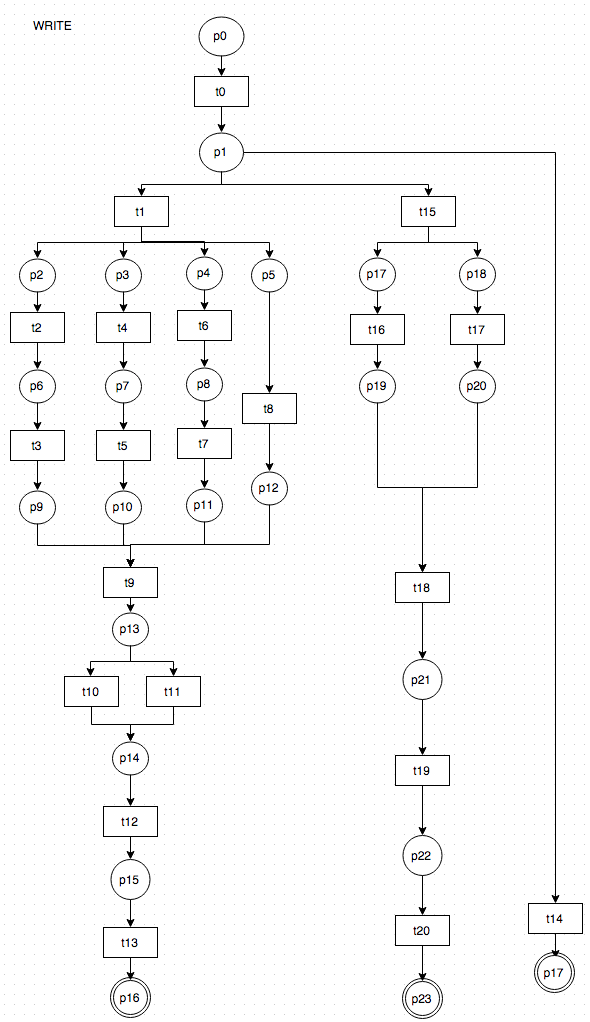
\includegraphics[width=3.7In]{figures/Fig5.png}}
%
%{\footnotesize
%\[
%\begin{array}{llll}
%msg_0: (&\mbox{ CPU1},&\mbox{writeReq},&\mbox{cache1   })\\       
%msg_1: (&\mbox{ cache1},&\mbox{ readExreq },&\mbox{Bus     })\\        
%msg_2: (&\mbox{ Bus},&\mbox{ readExreq},&\mbox{ cahce2 })\\  
%msg_3: (&\mbox{ cache2},&\mbox{readExreq},&\mbox{cpu2         })\\   
%msg_4: (&\mbox{ Bus},&\mbox{ readExreq},&\mbox{ cahce2           })\\  
%msg_5: (&\mbox{ cache2},&\mbox{readExreq},&\mbox{cpu2 })\\  
%msg_6: (&\mbox{ Bus},&\mbox{ readExreq},&\mbox{ cahce1       })\\     
%msg_7: (&\mbox{ cache1},&\mbox{readExreq},&\mbox{cpu1           })\\  
%msg_8: (&\mbox{ Bus},&\mbox{ readExreq},&\mbox{ Memory })\\  
%msg_9: (&\mbox{ true                                          })\\  
%msg_{10}: (&\mbox{ Memory},&\mbox{ readExres},&\mbox{ Bus        })\\  
%msg_{11}: (&\mbox{ cache2},&\mbox{ readExres},&\mbox{ Bus })\\  
%msg_{12}: (&\mbox{ Bus},&\mbox{ readExres},&\mbox{ cache1        })\\  
%msg_{13}: (&\mbox{ cache1},&\mbox{ writeRes},&\mbox{ CPU1         })\\  
%msg_{14}: (&\mbox{ cache1},&\mbox{ writeRes},&\mbox{ CPU1 })\\  
%msg_{15}: (&\mbox{ cache1},&\mbox{UpgradeReq             })\\  
%msg_{16}: (&\mbox{ Bus},&\mbox{ UpgradeReq},&\mbox{ cahce2      })\\   
%msg_{17}: (&\mbox{ Bus},&\mbox{ UpgradeReq},&\mbox{ Memory })\\  
%msg_{18}: (&\mbox{ cache2},&\mbox{UpgradeRes},&\mbox{ Bus     })\\  
%msg_{19}: (&\mbox{ Bus},&\mbox{ UpgradeRes},&\mbox{ cache1      })\\  
%msg_{20}: (&\mbox{ cache1},&\mbox{ WriteRes},&\mbox{ CPU1 })\\  
%\end{array}
%\]}
%\caption{Flow specification ($F_1$) of a cache coherent write operation initiated from CPU1}
%\label{write-flow}
%\end{figure}
%
%The LPN as shown in Fig.~\ref{write-flow} specifies a system flow where CPU1 initiates a memory write operation. In this flow, CPU1 initiates a memory write request to L1 Cache. Next, depends on whether the required data is included in cache1, the cache1 will generate three possible responses. First, the cache1 will send read exclusive request message msg2 to interconnect if data is not present in cache.; Or if the data is shared by CPU0, it will send upgrade message msg16 to interconnect to disable CPU0's ownership of this block of data, else if CPU1 has exclusive right of required data, cache1 will perform the write operation and sent an response message msg15 to CPU1. Afterwards, interconnect will sent request to all connected component (data cache and instruction cache of each CPU and memory). Once the interconnect obtains the response from either CPU0 or memory, it will generate a response message to cache1, then cache1 will generate a write response message msg14 (or msg 21 ) to CPU1. The flow is symmetric for CPU2.
%
%
%\begin{figure} 
%\centerline{
%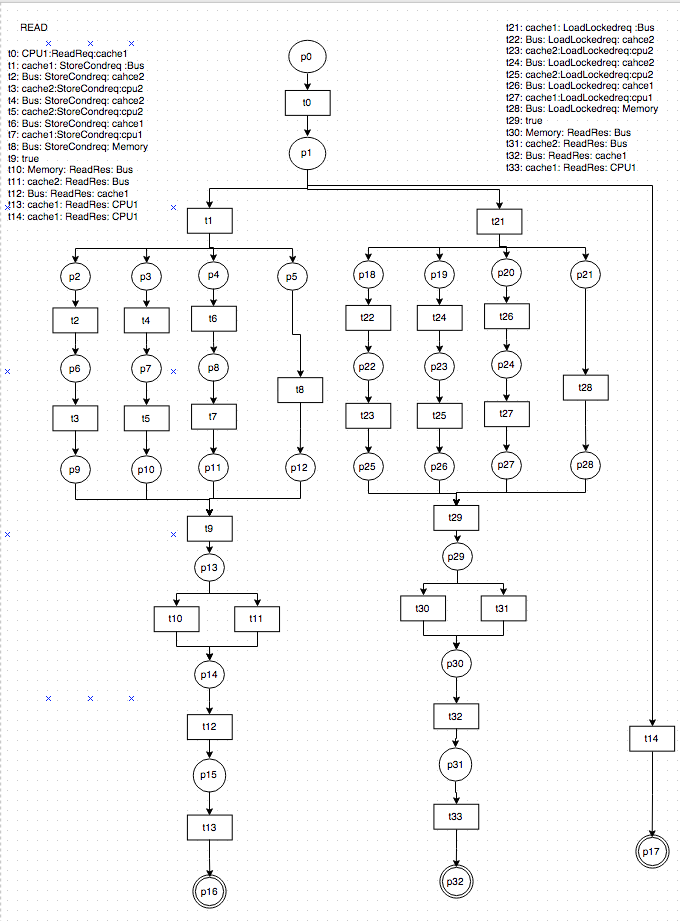
\includegraphics[width=4in]{figures/Fih6.png}}
%
%{\footnotesize
%\[
%\begin{array}{llll}
%t0: (&\mbox{ CPU1},&\mbox{ReadReq},&\mbox{cache1  })\\                   
%t1: (&\mbox{ cache1},&\mbox{ StoreCondreq },&\mbox{Bus })\\           
%t2: (&\mbox{ Bus},&\mbox{ StoreCondreq},&\mbox{ cahce2 })\\
%t3: (&\mbox{ cache2},&\mbox{StoreCondreq},&\mbox{cpu2       })\\      
%t4: (&\mbox{ Bus},&\mbox{ StoreCondreq},&\mbox{ cahce2           })\\ 
%t5: (&\mbox{ cache2},&\mbox{StoreCondreq},&\mbox{cpu2 })\\
%t6: (&\mbox{ Bus},&\mbox{ StoreCondreq},&\mbox{ cahce1     })\\       
%t7: (&\mbox{ cache1},&\mbox{StoreCondreq},&\mbox{cpu1           })\\ 
%t8: (&\mbox{ Bus},&\mbox{ StoreCondreq},&\mbox{ Memory })\\
%t9: (&\mbox{ true                                        })\\
%t10: (&\mbox{ Memory},&\mbox{ ReadRes},&\mbox{ Bus            })\\    
%t11: (&\mbox{ cache2},&\mbox{ ReadRes},&\mbox{ Bus })\\
%t12: (&\mbox{ Bus},&\mbox{ ReadRes},&\mbox{ cache1      })\\            
%t13: (&\mbox{ cache1},&\mbox{ ReadRes},&\mbox{ CPU1          })\\  
%t14: (&\mbox{ cache1},&\mbox{ ReadRes},&\mbox{ CPU1 })\\
%t21: (&\mbox{ cache1},&\mbox{ LoadLockedreq },&\mbox{Bus })\\     
%t22: (&\mbox{ Bus},&\mbox{ LoadLockedreq},&\mbox{ cahce2     })\\
%t23: (&\mbox{ cache2},&\mbox{LoadLockedreq},&\mbox{cpu2 })\\
%t24: (&\mbox{ Bus},&\mbox{ LoadLockedreq},&\mbox{ cahce2     })\\ 
%t25: (&\mbox{ cache2},&\mbox{LoadLockedreq},&\mbox{cpu2     })\\
%t26: (&\mbox{ Bus},&\mbox{ LoadLockedreq},&\mbox{ cahce1 })\\
%t27: (&\mbox{ cache1},&\mbox{LoadLockedreq},&\mbox{cpu1       })\\
%t28: (&\mbox{ Bus},&\mbox{ LoadLockedreq},&\mbox{ Memory     })\\
%t29: (&\mbox{ true })\\
%t30: (&\mbox{ Memory},&\mbox{ ReadRes},&\mbox{ Bus       })\\     
%t31: (&\mbox{ cache2},&\mbox{ ReadRes},&\mbox{ Bus    })\\
%t32: (&\mbox{ Bus},&\mbox{ ReadRes},&\mbox{ cache1 })\\
%t33: (&\mbox{ cache1},&\mbox{ ReadRes},&\mbox{ CPU1 })\\
%\end{array}
%\]}
%\caption{Flow specification ($F_2$) of a cache coherent read operation initiated from CPU1}
%\label{read-flow}
%
%\end{figure}
%The LPN specification as shown in Fig.~\ref{read-flow} captures the system flow where CPU1 initiate a memory read operation. Similar to memory write, CPU1 will first initiate a memory read request message msg1 to cache1. Cache1 can generate three possible responses. First, if the requested data is not in cache1, cache1 will generate an storeCondReq message msg2 to interconnect asking for data. Second, if the requested data is inside of cache1 but it's shared, cache1 will generate a upgrade request message msg22 to make sure it has the newest data; Last,  if cache1 has and data and it's not shared, it will generate a read response message msg15 to CPU1. Afterwards, interconnect will send corresponding request to all of its connected components. When interconnect receives the response, it will generate response message to cache1. Then cache1 will generate the read response message msg14 or msg34 to CPU1. This specification is also symmetric for CPU2.

%%%%%%%%%%%%%%%%%%%%%%%%%%%%%%%%%%%%%%%%%%%%%%%%%%%%%%%%%%%%%%%%%%%%%%
%\subsection{Results and Discussions}

We wrote two simple concurrent programs, one for each CPU,
 to exercise the flows.  They read numbers from a file,
perform some operations on these numbers, and store the
results back to the file.  How GEM5 supports shared memory
multi-threaded program execution is unclear.  Therefore,
no data are shared in both caches in this test.
Furthermore, GEM5 does not support true concurrency.  When
there are two programs running on the CPUs, GEM5 alternates
the executions between the two CPUs.  To simulate
asynchronous concurrency with the interleaving semantics,
those two simple programs are instrumented with
pseudo-blocking commands, one placed before each statement.
A pseudo blocking command includes a random number generator
that returns either $0$ or $1$ and a loop that only exits
when the returned random number is $0$.

%We produce a result file including all of the communication messages between every components from two simple programs running simultaneously on each CPU.  The program assigned to CPU1 read one file three times for one letter and writing one letter for three times to the same file. CPU2's program will do the same read and write functionalities to the same file, only difference is that CPU2 will write first and then read. One thing we should know about GEM5 is that even when we run these two programs concurrently, it will attempt to produce a concurrent result. The data we collected shows that it's not the real nondeterministic concurrency. What GEM5 did was it allowed two CPUs to execute its own instruction in turn, therefore the order was deterministic. Therefore, no matter how many times we ran the program, it produced the same result. We tried other virtual SoC platform softwares, and this was the best nondeterministic concurrency we can get. Even if this is slightly off with what the real chip should work, it still surve our purpose of testing the correctness of our algorithm.

\begin{table}[tb]
\caption{Runtime Results of Trace analysis. Time is in seconds and memory usage is in MB.}
\begin{center}
\begin{tabular}{|c|c|c|c|c|}
\hline
	&	F-Obs. & \begin{tabular}{c}P-Obs. \\ No Amb.\end{tabular} & \begin{tabular}{c}P-Obs. \\ Amb.~1\end{tabular} & \begin{tabular}{c}P-Obs. \\ Amb.~2\end{tabular} \\
\hline
\hline
Time & $3$ & $2.78$ & $896$ & $<1$\\
\hline
Mem & $12$ & $10$ & $420$ & $9$\\
\hline
	
\end{tabular}
\end{center}
\label{table-results}
\end{table}%

After this model is executed with the simple concurrent programs, 
the trace analysis is applied to traces with different observabilities
collected from this model.  The runtime results are shown in Table~\ref{table-results}.
The first column shows the results from analyzing the trace with the full
observability, while the next three show the result from 
analyzing traces with different partial observability assumptions.

In the first experiment, full observability is assumed.
After the SoC model finishes executing the program, there
are totally $343581$ messages collected in the trace file.
Not all of the messages are relevant to the flow
specification as many are used by GEM5 to initialize its
simulation environment.  After removing those irrelevant
messages, the number of messages in the trace file is to
reduced to $121138$.

The time taken to remove the irrelevant messages from the
trace is negligible.  The total runtime and the peak memory
taken by the trace analysis algorithm on the reduced
trace are 3 seconds and 12MB, respectively.  Only one flow execution
scenario is extracted, and 
Table~\ref{table-case-2} shows the number of flow instances contained in that
scenario for the six 
flows describing cache coherent operations initiated from both CPUs.
\begin{table}[tb]
\caption{The number of flow instances derived by the trace analysis with the full observability.}
\begin{center}
\begin{tabular}{|l|c|}
\hline
Flows & $\#$Instances \\
\hline
\hline
CPU1 Data Read			&  $17582$\\
CPU1 Instruction Read		&  $4002$\\
CPU1 Write				&  $3370$\\
\hline
CPU2 Data Read			&  $17386$\\
CPU2 Instruction Read		&  $3955$\\
CPU2 Write				&  $3308$\\
\hline
\end{tabular}
\end{center}
\label{table-case-2}
\end{table}%

In the second experiment, partial observability is taken into account
with the four monitors attached to the links between two CPUs and their
caches are disabled. Then, the trace is generated by the
remaining five monitors from the SoC model executing the
same program.  The new trace contains 15089 messages.  
Similarly, only one flow execution
scenario is extracted, and the numbers of the
flow instances contained in that execution scenario are
shown in Table~\ref{table-par-obs}.  From these results, the
numbers of the flow instances are dropped significantly
compared to the results extracted from the trace with the
full observability as shown in
Table~\ref{table-case-2}. This difference is due to that
some communications occurred in the system when executing
the program involve the CPUs and their corresponding caches
only, and the traffic on the links between the CPUs and
their corresponding caches is not observable. Therefore, the
instances of the flow specifications characterizing these
communications do not exist in the trace. In other words,
all extracted flow instances in Table~\ref{table-par-obs}
characterize the communications that pass through the memory
bus in the system model.  The runtime and memory usage as shown in
the third column in Table~\ref{table-results} are
similar to those for analyzing the trace of the full
observability.

\begin{table}[tb]
\caption{The number of flow instances derived by the trace analysis with certain monitors disabled.}
\begin{center}
\begin{tabular}{|l|c|}
\hline
Flows & $\#$Instances \\
\hline
\hline
CPU1 Data Read			&  $829$\\
CPU1 Instruction Read		&  $169$\\
CPU1 Write				&  $82$\\
\hline
CPU2 Data Read			&  $803$\\
CPU2 Instruction Read		&  $190$\\
CPU2 Write				&  $83$\\
\hline
\end{tabular}
\end{center}
\label{table-par-obs}
\end{table}%

In the third experiment, further partial observability is taken into consideration.  In this experiment, only the five links involving the memory bus are still considered.  However, an assumption is made that all events passing the same link are not distinguishable due to the limited observability.  The monitors are modified such that whenever an event is captured on one of the links, it dumps a set of events passing through the same link into the trace file.  Therefore, each line of the trace file corresponds to a set of events.  After applying the trace analysis to this trace,  a total of 13944 flow execution scenarios are extracted.    This large number, compared to the results from the first two experiments, is due to the ambiguous interpretation of the events with limited observability.  

The whole experiment takes about $15$ minutes and $420$~MB to finish as shown in column~4
in Table~\ref{table-results}, significantly higher than the numbers for analyzing traces where there is no ambiguity in the observed events.  This is due to the fact that a trace of ambiguous events is in fact a set of traces of original events, which lead to large numbers of execution scenarios either during or at the end of the analysis.  In this experiment, the peak number of execution scenarios during the analysis process is $70384$, many of which are invalid and removed eventually.  However, controlling the number of intermediate execution scenarios during the trace analysis is critical in order for the analysis to be tractable.  Here, insights from validators could help, but are not used in this experiment.   

As shown above, the ambiguous interpretation of events can lead to large numbers of intermediate and final execution scenarios, which not only make the trace analysis more time consuming but also make it difficult to gain insightful understanding from the derived execution scenarios.  Careful selection of what to observe may have big impact on results from the trace analysis.  In this last experiment, we relax the assumption made in the previous experiment such that the events passing each link are partitioned into two groups, one for read operations and one for write operations.  Similar to the assumption made in the previous experiment, events in the same group are assumed to be non-distinguishable.  The monitors are modified accordingly such that they output all events in the same group into the trace file if an event from that group is captured.  After the trace analysis on this new partially observed trace is finished, only one execution scenario is derived where the distribution of the numbers of flow instances is the same as those shown in Table~\ref{table-par-obs}.  The peak number of execution scenarios encountered during the trace analysis is $4$.  The total runtime and memory usage are negligible as shown in the last column in Table~\ref{table-results}.  Compared to the results from the previous experiment, the precision and the performance of the trace analysis are improved dramatically as a result of careful selection of observable events. 

%=====
\section{Related Work}

Our work is closely related to communication-centric and transaction based debug.  An early pioneering work is described in~\cite{Goossens2007NOCS}, which advocates the focus on observing activities on the interconnect network among IP blocks, and mapping these activities to transactions for better correlation between computations and communications.  Therefore, the communication transactions, as a result of software execution, provide an interface between computation and communication, and facilitate  system-level debug.  This work is extended in~\cite{Vermeulen2009VLSI-DAT,Goossens2009DATE}.  However, this line of work is focused on the network-on-chip (NoC) architecture for interconnect using the run/stop debug control method.  

A similar transaction-based debug approach is presented in~\cite{Gharehbaghi2012ISQED}.  Furthermore, it proposes an automated extraction of state machines at transaction level from  high level design models.  From an observed failure trace, it performs backtracking on this transaction level state machine to derive a set of transaction traces that lead to the observed failure state.  In the subsequent step, bounded model checking with the constraints on the internal variables is used to refine the set of transaction traces to remove the infeasible traces.  This approach requires user inputs to identify impossible transaction sequences, and may not find the states causing the failure if the transaction traces leading to the observed failure state is long.  Backtracking from the observed failure state requires pre-image computation, which can be computationally expensive.  A transaction-based online debug approach is proposed in~\cite{Dehbash2014} to address these issues.  This approach utilizes a transaction debug pattern specification language~\cite{Gharehbaghi2009ICCD} to define properties that transactions should meet.  These transaction properties are checked at runtime by programming debug units in the on-chip debug infrastructure, and the system can be stopped shortly after a violation is detected for any one of those properties.  In this sense, it can be viewed as the hardware assertion approaches in~\cite{Boule2007ISQED} elevated to the transaction level. 

In~\cite{Singerman2011DAC}, a coherent workflow is described where the result from the pre-silicon validation stage can be carried over to the post-silicon stage to improve efficiency and productivity of post-silicon debug.  This workflow is centered on a repository of system events and simple transactions defined by architects and IP designers.  It spans across a wide spectrum of the post-silicon validation including DFx instrumentation, test generation, coverage, and debug.  The DFx instruments are automatically inserted into the design RTL code driven by the defined transactions.  This instrumentation is optimized for making a large set of events and transactions observable.   Test generation is also optimized to generate only the necessary but sufficient tests to allow all defined transactions to be exercised.   Moreover, coverage for post-silicon validation is now defined at the abstract level of events and transactions rather than the raw signals, and thus can be evaluated more efficiently.  In~\cite{Abarbanel2014DAC}, a model at an even higher-level of abstraction, {\em flows}, is proposed.  Flows are used to specify more sophisticated cross-IP transactions such as power management, security, etc, and to facilitate reuse of the efforts of the architectural analysis to check HW/SW implementations. 


%
%--
\section{Conclusion}

This paper presents a method for post-silicon validation by interpreting observed raw signal traces at the level of system flow specifications.  The derived flow execution scenarios provide more structured information on system operations, which is more understandable to system validators.   This information can help to locate design defects more easily, and also provides a measurement of validation coverage.  

Due to partial observability, this approach may derive a large number of different flow execution scenarios for a given signal trace.  Insights from system validators can help to eliminate some false scenarios due to the partial observability.  An interesting future direction is formalization of the validators' insights using temporal logic on flows so that the validators can express their intents more precisely and concisely. 

The trace analysis approach presented in this paper needs to be iterated with different observations selected in different iterations in order to eliminate the false scenarios and to root cause system failures as quickly as possible.  The observation selection and stitching signal traces of different observations together for the above goal will also be pursued in the future.




% conference papers do not normally have an appendix


% use section* for acknowledgement
%\section*{Acknowledgment}
%
%
%The authors would like to thank...
%




% trigger a \newpage just before the given reference
% number - used to balance the columns on the last page
% adjust value as needed - may need to be readjusted if
% the document is modified later
%\IEEEtriggeratref{8}
% The "triggered" command can be changed if desired:
%\IEEEtriggercmd{\enlargethispage{-5in}}

% references section

% can use a bibliography generated by BibTeX as a .bbl file
% BibTeX documentation can be easily obtained at:
% http://www.ctan.org/tex-archive/biblio/bibtex/contrib/doc/
% The IEEEtran BibTeX style support page is at:
% http://www.michaelshell.org/tex/ieeetran/bibtex/
\bibliographystyle{IEEEtran}
% argument is your BibTeX string definitions and bibliography database(s)
\bibliography{SoC}
%
% <OR> manually copy in the resultant .bbl file
% set second argument of \begin to the number of references
% (used to reserve space for the reference number labels box)
%\begin{thebibliography}{1}
%
%\bibitem{IEEEhowto:kopka}
%H.~Kopka and P.~W. Daly, \emph{A Guide to \LaTeX}, 3rd~ed.\hskip 1em plus
%  0.5em minus 0.4em\relax Harlow, England: Addison-Wesley, 1999.
%
%\end{thebibliography}




% that's all folks
\end{document}


